%%%%%%%%%%%%%%%%%%%%%%%%%%%%%%%%%%%%%%%%%%%%%%%%%%%%%%%%%%%%%%%%%%%%%%%%%%%%%%%
%% Descr:       Vorlage für Berichte der DHBW-Karlsruhe
%% Author:      Prof. Dr. Jürgen Vollmer, juergen.vollmer@dhbw-karlsruhe.de
%% $Id: bericht.tex,v 1.24 2018/10/23 09:10:06 vollmer Exp $
%%  -*- coding: utf-8 -*-
%%%%%%%%%%%%%%%%%%%%%%%%%%%%%%%%%%%%%%%%%%%%%%%%%%%%%%%%%%%%%%%%%%%%%%%%%%%%%%%

\documentclass[
   ngerman          % neue deutsche Rechtschreibung
  ,a4paper          % Papiergrösse
% ,twoside          % Zweiseitiger Druck (rechts/links)
% ,10pt             % Schriftgrösse
  ,11pt
% ,12pt
  ,pdftex
%  ,disable         % Todo-Markierungen auschalten
]{report}

% Bitte die Codierung Ihrer Dateien auswählen:
% \usepackage[latin1]{inputenc}    % Für UNIX mit ISO-LATIN-codierten Dateien
% \usepackage[applemac]{inputenc}  % Für Apple Mac
% \usepackage[ansinew]{inputenc}   % Für Microsoft Windows
\usepackage[utf8]{inputenc}        % UTF-8 codierte Dateien
                                   % Dieses Dokument ist unter Unix erstellt, daher
                                   % wird diese Input-Codierung benutzt.

\usepackage{bericht}

%%%%%%%%%%%%%%%%%%%%%%%%%%%%%%%%%%%%%%%%%%%%%%%%%%%%%%%%%%%%%%%%%%%%%%%%%%%%%%%
%% Angaben zur Arbeit
%%%%%%%%%%%%%%%%%%%%%%%%%%%%%%%%%%%%%%%%%%%%%%%%%%%%%%%%%%%%%%%%%%%%%%%%%%%%%%%

\newcommand{\Autor}{Mikka Jenne und Simon Leitl}
\newcommand{\MatrikelNummer}{2062885, 7068806}
\newcommand{\Kursbezeichnung}{tinf17b4}

\newcommand{\FirmenName}{cjt Systemsoftware AG}
\newcommand{\FirmenStadt}{Karlsruhe}
%\newcommand{\FirmenLogoDeckblatt}{\fbox{
\includegraphics[width=3cm]{lion}}}

% Falls es kein Firmenlogo gibt:
\newcommand{\FirmenLogoDeckblatt}{}

%\newcommand{\BetreuerFirma}{Titel Vorname Nachname}
\newcommand{\BetreuerDHBW}{Prof. Dr. Kai Becher}

%%%%%%%%%%%%%%%%%%%%%%%%%%%%%%%%%%%%%%%%%%%%%%%%%%%%%%%%%%%%%%%%%%%%%%%%%%%%%%%%%%%%%

% Wird auf dem Deckblatt und in der Erklärung benutzt:
%\newcommand{\Was}{Projekt-/Studien-/Bachleorarbeit}
%\newcommand{\Was}{Projektrarbeit}
\newcommand{\Was}{Studienarbeit}
%\newcommand{\Was}{Bachleorarbeit}

%%%%%%%%%%%%%%%%%%%%%%%%%%%%%%%%%%%%%%%%%%%%%%%%%%%%%%%%%%%%%%%%%%%%%%%%%%%%%%%%%%%%%

\newcommand{\Titel}{Entwicklung einer Software zur Schaltplanerstellung in der Elektrotechnik}
\newcommand{\AbgabeDatum}{01. Juni 2020}

\newcommand{\Dauer}{12 Wochen}

% \newcommand{\Abschluss}{Bachelor of Engineering}
\newcommand{\Abschluss}{Bachelor of Science}

\newcommand{\Studiengang}{Informatik}
% \newcommand{\Studiengang}{Informatik / Angewandte Informatik}

\hypersetup{%%
  pdfauthor={\Autor},
  pdftitle={\Titel},
  pdfsubject={\Was}
}

%%%%%%%%%%%%%%%%%%%%%%%%%%%%%%%%%%%%%%%%%%%%%%%%%%%%%%%%%%%%%%%%%%%%%%%%%%%%%%%

% Wenn \includeonly{..} benutzt wird, werden nur diese Kaptitel ausgegeben.
%\includeonly{
 % abk
 %,kapitel1
 %,kapitel2
 %,kapitel3
 %,systementwurf
 %,changelog
%}

%%%%%%%%%%%%%%%%%%%%%%%%%%%%%%%%%%%%%%%%%%%%%%%%%%%%%%%%%%%%%%%%%%%%%%%%%%%%%%%

% Benutzt man das "biblatex"-Paket, dann muß das hier stehen:
% siehe auch die mit BIBLATEX markierten Zeilen in bericht.sty
\bibliography{bericht}

\begin{document}

%%%%%%%%%%%%%%%%%%%%%%%%%%%%%%%%%%%%%%%%%%%%%%%%%%%%%%%%%%%%%%%%%%%%%%%%%%%%%%%%

\begin{titlepage}
\begin{center}
\vspace*{-2cm}
\FirmenLogoDeckblatt\hfill
\includegraphics[width=4cm]{dhbw-logo}\\[2cm]
{\Huge \Titel}\\[1cm]
{\Huge\scshape \Was}\\[1cm]
{\large für die Prüfung zum}\\[0.5cm]
{\Large \Abschluss}\\[0.5cm]
{\large des Studienganges \Studiengang}\\[0.5cm]
{\large an der}\\[0.5cm]
{\large Dualen Hochschule Baden-Württemberg Karlsruhe}\\[0.5cm]
{\large von}\\[0.5cm]
{\large\bfseries \Autor}\\[1cm]
{\large Abgabedatum \AbgabeDatum}
\vfill
\end{center}
\begin{tabular}{l@{\hspace{2cm}}l}
Bearbeitungszeitraum	         & \Dauer 			\\
Matrikelnummer	                 & \MatrikelNummer		\\
Kurs			         & \Kursbezeichnung		\\
Ausbildungsfirma	         & \FirmenName			\\
			         & \FirmenStadt			\\
%Betreuer der Ausbildungsfirma	 & \BetreuerFirma		\\
Gutachter der Studienakademie	 & \BetreuerDHBW		\\
\end{tabular}
\end{titlepage}
 
%%%%%%%%%%%%%%%%%%%%%%%%%%%%%%%%%%%%%%%%%%%%%%%%%%%%%%%%%%%%%%%%%%%%%%%%%%%%%%%

%%%%%%%%%%%%%%%%%%%%%%%%%%%%%%%%%%%%%%%%%%%%%%%%%%%%%%%%%%%%%%%%%%%%%%%%%%%%%%%
%% Descr:       Vorlage für Berichte der DHBW-Karlsruhe, Erklärung
%% Author:      Prof. Dr. Jürgen Vollmer, vollmer@dhbw-karlsruhe.de
%% $Id: erklaerung.tex,v 1.11 2020/03/13 14:24:42 vollmer Exp $
%% -*- coding: utf-8 -*-
%%%%%%%%%%%%%%%%%%%%%%%%%%%%%%%%%%%%%%%%%%%%%%%%%%%%%%%%%%%%%%%%%%%%%%%%%%%%%%%

% In Bachelorarbeiten muss eine schriftliche Erklärung abgegeben werden.
% Hierin bestätigen die Studierenden, dass die Bachelorarbeit, etc.
% selbständig verfasst und sämtliche Quellen und Hilfsmittel angegeben sind. Diese Erklärung
% bildet das zweite Blatt der Arbeit. Der Text dieser Erklärung muss auf einer separaten Seite
% wie unten angegeben lauten.

\newpage
\thispagestyle{empty}
\begin{framed}
\begin{center}
\Large\bfseries Erklärung
\end{center}
\medskip
\noindent
% siehe §5(3) der \enquote{Studien- und Prüfungsordnung DHBW Technik} vom 29.\,9.\,2017 und Anhang 1.1.13
Ich versichere hiermit, dass ich meine \Was mit dem Thema:
\enquote{\Titel}
selbstständig verfasst und keine anderen als die angegebenen Quellen und Hilfsmittel benutzt habe. Ich versichere zudem, dass die eingereichte elektronische Fassung mit der gedruckten Fassung übereinstimmt.
\vspace{3cm}
\noindent
\underline{\hspace{4cm}}\hfill\underline{\hspace{6cm}}\\
Ort~~~~~Datum\hfill Unterschrift\hspace{4cm}
\end{framed}

\vfill
\emph{Sofern  vom Dualen Partner ein Sperrvermerk gewünscht wird, ist folgende Formulierung
zu verwenden:}
\begin{framed}
\begin{center}
\Large\bfseries Sperrvermerk
\end{center}
\medskip
\noindent
Der Inhalt dieser Arbeit darf weder als Ganzes noch in Auszügen Personen
außerhalb des Prüfungsprozesses und des Evaluationsverfahrens zugänglich gemacht
werden, sofern keine anderslautende Genehmigung vom Dualen Partner vorliegt.
\end{framed}

%%%%%%%%%%%%%%%%%%%%%%%%%%%%%%%%%%%%%%%%%%%%%%%%%%%%%%%%%%%%%%%%%%%%%%%%%%%%%%%
\endinput
%%%%%%%%%%%%%%%%%%%%%%%%%%%%%%%%%%%%%%%%%%%%%%%%%%%%%%%%%%%%%%%%%%%%%%%%%%%%%%%


%%%%%%%%%%%%%%%%%%%%%%%%%%%%%%%%%%%%%%%%%%%%%%%%%%%%%%%%%%%%%%%%%%%%%%%%%%%%%%%

\begin{abstract}
  Computer sind heutzutage allgegenwärtig.
  \\Kaum ein Unternehmen arbeitet ohne computergesteuerte Unterstützung, 
  sei es das Schreiben einer Rechnung in einem mittelständischen Unternehmen, das Verwalten von einzelnen Arbeitsprozessen oder 
  die Unterstützung bei einzelnen Arbeitsschritten. Speziell im Elektrotechnischen Bereich gibt es heute noch Prozesse die hinsichtlich
  der physischen und digitalen Welt stark voneinander getrennt sind, z.B. das Zeichnen von Schaltplänen und die
  digitale Erfassung von Messwerten, die über Programme verwaltet werden können.
  \\Das Ziel dieser Arbeit ist es, die physische Welt durch die Möglichkeit der digitalen Zeichnung von Gebäudeschaltplänen
  zu erweitern. Für den Gebrauch designed, wird auf eine Verbesserung sowie auf die Transparenz von solchen Schaltplänen gezielt,
  um so weitere essentielle Informationen zu Gebäuden zu erhalten. Da die händische Zeichnung meist aufwändig, kostenintensiv ist und keiner Norm entspricht,
  soll durch die Digitalisierung dieses Prozesses Abhilfe geschaffen werden. Durch Nutzung neuester Technologien im Bereich Desktopanwendungen
  und des Einsatzes einer einheitlichen Zeichenstruktur sollte diese Applikation für den Otto Normalverbraucher leicht nutzbar sein.  
\end{abstract}

\newpage
\tableofcontents           % Inhaltsverzeichnis hier ausgeben
\listoffigures             % Liste der Abbildungen
%\listoftables              % Liste der Tabellen
\lstlistoflistings         % Liste der Listings
%\listofequations           % Liste der Formeln
% Jetzt kommt der "eigentliche" Text
%%%%%%%%%%%%%%%%%%%%%%%%%%%%%%%%%%%%%%%%%%%%%%%%%%%%%%%%%%%%%%%%%%%%%%%%%%%%%%
%% Descr:       Vorlage für Berichte der DHBW-Karlsruhe, Datei mit Abkürzungen
%% Author:      Prof. Dr. Jürgen Vollmer, vollmer@dhbw-karlsruhe.de
%% $Id: abk.tex,v 1.4 2017/10/06 14:02:03 vollmer Exp $
%% -*- coding: utf-8 -*-
%%%%%%%%%%%%%%%%%%%%%%%%%%%%%%%%%%%%%%%%%%%%%%%%%%%%%%%%%%%%%%%%%%%%%%%%%%%%%%%

\chapter*{Abkürzungsverzeichnis}                   % chapter*{..} -->   keine Nummer, kein "Kapitel"
						         % Nicht ins Inhaltsverzeichnis
% \addcontentsline{toc}{chapter}{Akürzungsverzeichnis}   % Damit das doch ins Inhaltsverzeichnis kommt

% Hier werden die Abkürzungen definiert
\begin{acronym}[DHBW]
  % \acro{Name}{Darstellung der Abkürzung}{Langform der Abkürzung}
 \acro{Abk}[Abk.]{Abkürzung}
 \acro{API}[API]{Application Programming Interface}
 \acro{AR}[AR]{Augmented Reality}
 \acro{DBMS}[DBMS]{Datenbank-Management-System}
 %\acro{ER}[ER]{deutsch erweiterte Realität}
 \acro{EKF}[EKF]{Erweiterter Kalman Filter}
 \acro{ERM}[ERM]{Entity-Relationship-Modell}
 \acro{Fraunhofer IOSB}[IOSB]{Fraunhofer Institut für Optronik, Systemtechnik und Bildauswertung IOSB}
 \acro{GPS}[GPS]{Global Positioning System}
 \acro{HMD}[HMD]{Head-Mounted Display}
 \acro{ICP}[ICP]{Iterativ Closest Point}
 \acro{IMU}[IMU]{Inertial Measurement Unit}
 \acro{INS}[INS]{Inertial Navigation System}
 \acro{IoT}[IoT]{Internet of Things, dt. Internet der Dinge}
 \acro{KIT}[KIT]{Forschungszentrum Karlsruhe}
 \acro{MEMS}[MEMS]{Micro-Electro-Mechanical Systems}
 \acro{MR}[MR]{Mixed Reality}
 \acro{MVC}[MVC]{Model View Controller}
 \acro{SDK}[SDK]{Software Development Kit}
 \acro{SLAM}[SLAM]{Simultanious Localization And Mapping}
 \acro{SQL}[SQL]{Structured Query Language}
 \acro{TOF}[TOF]{Time of flight}
 \acro{UX}[UX]{User-Excperience, dt. Nutzererfahrung und Nutzererlebnis}
 \acro{UC}[UC]{Use Case}
 \acro{UCs}[UCs]{Use Cases}
 \acro{UI}[GUI]{Graphical User Interface, dt. Benutzeroberfläche}
 \acro{VR}[VR]{Virtual Reality}
 \acro{WMR}[WMR]{Windows Mixed Reality}
 % Folgendes benutzen, wenn der Plural einer Abk. benöigt wird
 % \newacroplural{Name}{Darstellung der Abkürzung}{Langform der Abkürzung}
 \newacroplural{Abk}[Abk-en]{Abkürzungen}


 \acro{H2O}[\ensuremath{H_2O}]{Di-Hydrogen-Monoxid}

 % Wenn neicht benutzt, erscheint diese Abk. nicht in der Liste
 \acro{NUA}{Not Used Acronym}
\end{acronym}
              % Abkürzungsverzeichnis
%%%%%%%%%%%%%%%%%%%%%%%%%%%%%%%%%%%%%%%%%%%%%%%%%%%%%%%%%%%%%%%%%%%%%%%%%%%%%%
%% Descr:       Vorlage für Berichte der DHBW-Karlsruhe, Ein Kapitel
%% Author:      Prof. Dr. Jürgen Vollmer, vollmer@dhbw-karlsruhe.de
%% $Id: kapitel1.tex,v 1.17 2018/10/23 08:58:41 vollmer Exp $
%% -*- coding: utf-8 -*-
%%%%%%%%%%%%%%%%%%%%%%%%%%%%%%%%%%%%%%%%%%%%%%%%%%%%%%%%%%%%%%%%%%%%%%%%%%%%%%%

\chapter{Einleitung}
In diesem Teil der Arbeit wird auf die Motivation des Themas eingegangen. 
Die Aufgabenstellung genau erläutert und sowohl die Ziele als auch der Aufbau der Arbeit dargelegt.
\section{Motivation}
Die herkömmlichen Schaltpläne von Gebäuden, Schaltschränken oder Maschinen werden aus der Historie heraus per Hand auf normales Papier
gezeichnet. Der Elektrotechniker oder gar ein Architekt nimmt Zeit in Anspruch einen solchen Plan detailgetreu und 
nach Maßstab zu zeichnen. Diese Arbeit ist sehr zeitintensiv und preislich sehr teuer. Zudem können handschriftliche Änderungen
das Dokument unübersichtlich machen, bzw. müsste bei jeder Änderung ein neuer Plan ausgefertigt werden. 
\\Aus diesen Gründen wird eine Zeichnung meistens vernachlässigt, wobei es für Zukünftige Arbeiten,
z.B. Sanierungen, Ausbauten o.ä. essentiell ist. Um diesem fatalen Fehler, den Plan zu vermeiden, entgegenzuwirken wurden Ideen und
Vorschläge gesammelt, wie dieser Prozess deutlich einfacher und ressourcenschonender vonstattengehen könnte.
\\
\linebreak
Diese Problemstellung der realen Welt führte dazu diese Aufgabe in Angriff zu nehmen und diesen Prozess zu modernisieren.
Mit dem Gedanken und der Intension der Digitalisierung in der Elektrotechnik wurden Überlegungen getätigt diese Modernisierung
umzusetzen.
\linebreak
\linebreak
Ein motivierender Aspekt dieses Vorgehens ist, dass die auf Papier gezeichneten Dokumente verloren gehen oder physische Schäden erleiden können
und so unbrauchbar werden. Durch die Digitalisierung des Verfahrens sind diese Aspekte ausgeschlossen und sind deutlich vielseitiger.
\linebreak
\linebreak
Im Zeitalter der Industrie 4.0, bei der der Schwerpunkt auf Digitalisierung liegt, war es leicht eine Idee zu generieren die 
standardmäßige Schaltpläne in dem Zeichnungs- und Ausarbeitungsprozess verbessert und ein bekanntest Problem löst.
Sowohl in zeitlicher und kostspieliger Hinsicht als auch die Übersichtlichkeit
solcher Dokumente kann enorm gesteigert werden. Veränderungen keine neue Zeichnung anzufertigen, sondern können in der bestehenden
Datei schnell und einfach ausgebessert werden. 
\newpage
\section{Aufgabenstellung}
Es soll ein Konzept für eine Software erstellt werden, welches erlaubt Schaltpläne digital zu zeichnen, anzuzeigen, 
flexibel zu ändern und alle wichtigen Informationen zu Verfügung zu stellen. 
\\ Dieses ausgearbeitete Konzept soll einen modularen Ansatz verfolgen, um in Zukunft beliebig erweiterbar zu sein
und die Integration von neuen Features zu gewährleisten. Nach Erstellung des Konzepts und der definierten Software-Architektur
soll der Grundbaustein der Applikation gelegt und gefestigt werden, indem die Grundfunktion implementiert und getestet werden.
\\Die Grundfunktionen werden in folgendem kurz aufgelistet, um einen groben Überblick zu verschaffen.
\begin{itemize}
    \item Startmenü - Übersicht
    \begin{itemize}
        \item Erstellen eines Schaltplans
        \item Öffnen einer vorhandenen Schaltplan-Datei
        \item Weiterarbeiten an einer Schaltplan-Datei
    \end{itemize}
    \item Editor
    \begin{itemize}
        \item Grundgerüst Zeichen (Grundriss, Türen, etc.)
        \item Leitungen Zeichen (Größe, Stärke der Leitung)
        \item Mögliche Komponenten einfügen (Steckdose, Lichtschalter, etc.) 
        \item Anzeige von Informationen zu Komponenten und Leitungen
        \item Legende zum Verständnis und zur Übersicht der einzelnen Zeichenkomponenten
    \end{itemize}
    
\end{itemize}
Die obenstehenden Punkte sehen die Grundfunktionen vor und werden in drei große Teilbereiche, wie zu erkennen, abgegrenzt. 
Das Design und der allgemeine Aufbau wird in folgenden Kapiteln genauer erläutert und anhand von Bildern,
Mockups und Diagrammen dargestellt.
\linebreak
\linebreak
Der Hauptaugenmerk dieser Aufgabe, bzw. der Problemstellung liegt darin die Möglichkeit zu schaffen
einen Schaltplan rentabel und einfach zu digitalisieren, um den Einsatz von Schaltplanzeichnungen erneut zu verbreiten beziehungsweise
zu modernisieren. 
\newpage
\section{Aufbau der Arbeit}
Nach den oben genannten einleitenden Informationen widmet sich das Kapitel 2 den essentiellen und wichtigsten Grundlagen dieser Arbeit.
Zu Anfang werden allgemein gültige Grundlagen zur Digitalisierung in der Gebäudetechnik (2.1) offenbart, um Kontexte zur Arbeit im Allgemeinen
zu verstehen, gefolgt von einer Einführung in die modulare Software Architektur (2.2) zum Ende des Kapitels.
\linebreak
\linebreak
Anschließend auf Kapitel 2 wird in Kapitel 3 auf die verwendeten Technologien und Tools eingegangen. Mit Windows Presentation Foundation
(3.1) wird erläutert was es damit auf sich hat und welche Programmiersprache diese Technologie sich zu eigen macht. In (3.2) wird das MVVM-Pattern
genauestens erklärt, was es bedeutet, wie und warum es angewendet wird. Das Windows eigene System.Drawing, welches zum 
Zeichnen der Schaltpläne verwendet wird in (3.3) aufgeführt.
\linebreak
\linebreak
Nach den verwendeten Technologien geht es in Kapitel 4 um den eigentlichen Systementwurf, zum einen um das Architekturkonzept (4.1)
und zum anderen um das Softwarekonzept (4.2). Dabei wird auch detailliert auf das Aussehen eingegangen und die graphischen Benutzeroberflächen, GUIs,
anhand mehreren Mockups dargelegt.
\\
\linebreak
In Kapitel 5 wird genauestens auf die praktische Umsetzung und Implementierung der vier definierten Use Cases eingegangen, 
die im einzelnen kurz chronologisch aufgeführt werden.
\begin{itemize}
    \item Startmenü (5.1)
    \item Toolbox (5.2)
    \item Zeichenfläche (5.3)
\end{itemize}
Die letzten zwei Kapitel, Ereignis (6) und Ausblick (7), runden die Dokumentation ab und schließen die Arbeit. Das Ergebnis wird hierbei
analysiert und Verbesserungsvorschläge angemerkt. 
\\ Der Ausblick gibt Aufschluss darüber welche möglichen Erweiterungsmöglichkeiten es gibt und wie die Zukunft dieser Arbeit möglicherweise aussehen könnte.

%%%%%%%%%%%%%%%%%%%%%%%%%%%%%%%%%%%%%%%%%%%%%%%%%%%%%%%%%%%%%%%%%%%%%%%%%%%%%
%% Descr:       Vorlage für Berichte der DHBW-Karlsruhe, Ein Kapitel
%% Author:      Prof. Dr. Jürgen Vollmer, vollmer@dhbw-karlsruhe.de
%% $Id: kapitel2.tex,v 1.5 2017/10/06 14:02:51 vollmer Exp $
%%  -*- coding: utf-8 -*-
%%%%%%%%%%%%%%%%%%%%%%%%%%%%%%%%%%%%%%%%%%%%%%%%%%%%%%%%%%%%%%%%%%%%%%%%%%%%%%%

\chapter{Grundlagen}
\label{chap:Grundlagen}
In diesem Kapitel werden die für diese Bachelorarbeit notwendigen Grundlagen geschaffen, um ein fundiertes Wissen und Verständnis 
über verwendete Technologien zu schaffen. Auf alle diese Informationen und Voraussetzungen wird im Folgenden eingegangen, um nachfolgende 
Konzeption und Umsetzung besser zu verstehen.

\section{Augmented Reality}
\label{chap:Augmented Reality}
Eine der wichtigsten Grundlagen dieser Arbeit ist das Verständnis des Begriffs der Augmented Reality.
\\ 
\acl{AR}, deutsch erweiterte Realität, ist eine durch den Computer gestützte Erweiterung der Realität, bzw. der menschlichen 
Wahrnehmung. Es ermöglicht dem Nutzer die reale Welt mit Überlagerung oder Zusammensetzung virtueller Objekte und visueller Informationen
zu sehen. Mittels einer Art Overlay werden diese Objekte und Informationen über die reale Welt gelegt und dem Nutzer zur Verfügung gestellt. 
Allgemein soll damit dem Nutzer ein weit gefächerter Überblick verschafft werden und Hilfestellung leisten, aber den Nutzer in keinerlei 
Interaktion mit der Umgebung einschränken. Die Definition, welche sich in der Wissenschaft weitestgehend durchgesetzt und etabliert hat ist 
die Definition nach Azuma aus dem Jahre 1997.
\begin{quote}
    „Augmented Reality (AR) is a variation of Virtual Environments (VE), or Virtual Reality as it is more commonly called. VE 
    technologies completely immerse a user inside a synthetic environment. While immersed, the user cannot see the real world around him. 
    In contrast, AR allows the user to see the real world, with virtual objects superimposed upon or composited with the real world. 
    Therefore, AR supplements reality, rather than completely replacing it.“ \cite{azuma.1997a}
\end{quote}
Ein Augmented Reality System verfügt nach \cite{azuma.1997a} über folgende drei charakteristische Merkmale: 
\begin{enumerate}
    \item Es kombiniert Realität und Virtualität.
    \item Es ist interaktiv in Echtzeit.
    \item Die virtuellen Inhalte sind im 3D registriert.
\end{enumerate}
Das erste genannte Merkmal kombiniert die reale Welt mit dem oben genannten Overlay, der Überlagerung der Realität um künstliche virtuelle 
Objekte und visuelle Informationen. Dies bedeutet, der Nutzer nimmt die reale Umgebung gleichzeitig mit den darin liegenden virtuellen 
Objekten als ein Ganzes wahr. Daraus resultiert die Interaktion von virtuellen Objekten und Informationen mit der realen Welt in Echtzeit, 
damit sie als Teil der Realität registriert werden können. Das dritte Merkmal umfasst die Darstellung von Objekten als scheinbar reales 
Objekt. Mit dem letzt genannten Merkmal wird das Ziel verfolgt die projizierten, bzw. nicht realen Teile täuschend echt in die Umgebung zu 
integrieren.
\\ 
\linebreak  
%Darüber hinaus sind die virtuellen Inhalte in 3D (d. h. geometrisch) registriert. Dies bedeutet nichts anderes, als dass in einer 
%AR-Umgebung ein virtuelles Objekt scheinbar einen festen Platz in Realität hat und diesen, sofern es nicht durch eine Benutzerinteraktion 
%verändert wird oder sich z. B. in Form einer Animation selbst verändert, auch beibehält. Mit anderen Worten: Es verhält sich aus Nutzersicht 
%genauso, wie ein reales Objekt, was sich an diesem Ort befinden würde
Eine etwas allgemein formuliertere Definition ist die nach \cite{springer.2019s}, welche die drei charakteristischen Merkmale besonders 
aufgreift:
\begin{quote}
    „Augmentierte Realität (AR) ist eine (unmittelbare und interaktive) um virtuelle Inhalte (für beliebige Sinne) angereicherte Wahrnehmung der 
    realen Umgebung in Echtzeit, welche sich in ihrer Ausprägung und Anmutung soweit wie möglich an der Realität orientiert, sodass im 
    Extremfall (so dies gewünscht ist) eine Unterscheidung zwischen realen und virtuellen (Sinnes-) Eindrücken nicht mehr möglich ist.„ \cite{springer.2019s}
\end{quote}
Diese Definition nimmt sich als Grundlage die oben aufgeführte Definition nach \cite{azuma.1997a}.
\\ 
\linebreak
Der Author L. Frank Baum \cite{frankbaum.1856m} verkündete die ersten Ideen und Gedanken einer Augmented Reality Anwendung in 
\textit{„The Master Key“} \cite{masterkey.1996f}. Eine erste tatsächliche Realisierung eines Augmented Reality Systems erfolgte erst über 
60 Jahr später. Ivan Edward Sutherland \cite{sutherlandbio.1938m} stellte sein Projekt 1968 an der University of Utah vor. Dabei handelte es 
sich um ein sogenanntes \textit{\ac{HMD}}. Ziel dieser Entwicklung war weniger das Erweitern der Realität, sondern dreidimensionale 
Illusionen zu erzeugen die reale Objekte mit einer einfachen Grafik in Echtzeit überlagert. %\cite{display.1965f}
Trotz dessen gilt er als erste Person mit der Vision, einen Nutzer in realer Umgebung mit virtuellen Objekten interagieren zu lassen.
\\ 
Anfang der 90er Jahre prägten zwei Forscher, Thomas P. Caudell und David W. Mizell, den Begriff der Augmented Reality durch ein Pilotprojekt
bei Boeing. Das Projekt diente dazu Informationen in das Gesichtsfeld über eine Brille einzusetzen, um Arbeitern das Verlegen von Kabeln im und um das 
Flugzeug zu erleichtern. Nach dieser bahnbrechenden Erfindung begann eine stetige Weiterentwicklung der Technologie. Im Jahre 1999 wurde 
von Hirokazu Kato und Mark Billinghurst \textit{ARToolKit}, ein Computer-Vision-basiertes Tracking für AR, veröffentlicht und „löste eine 
große Welle an Forschungsarbeiten auf der ganzen Welt aus.“ \cite{springer.2019s} 
\begin{quote}
    We describe an augmented reality conferencing system which uses the overlay of virtual images on the real world. Remote collaborators 
    are represented on Virtual Monitors which can be freely positioned about a user in space. Users can collaboratively view and interact 
    with virtual objects using a shared virtual whiteboard. This is possible through precise virtual image registration using fast and 
    accurate computer vision techniques and HMD calibration. We propose a method for tracking fiducial markers and a calibration method 
    for optical see-through HMD based on the marker tracking. \cite{artoolkitsheet.1999o}
\end{quote}
Dieser Ausschnitt war der grundlegende Baustein des Durchbruchs dieser Technologie und den vorangestellten Forschungen und eine fundierte 
Grundlage für alle Forschungen und Entwicklungen die darauf folgten. 
\\ 
Heutzutage dreht sich die Entwicklung um mobile AR, welche durch die anfängliche Revolution von \textit{ARToolkit} und die darauf entstehenden 
Entwicklungen und Produktionen von großen Firmen, wie z.B. Google, Microsoft, Apple und Facebook entstand. Die zuletzt große Bewegung in dem 
Bereich der AR waren die Vorstellungen großer Software-Plattformen für mobile \acs{AR}-Applikationen. Durch \textit{Apple's ARKit} und \textit{Google's ARCore} 
kamen im Jahr 2017 zwei moderne und innovative Frameworks auf den Markt, die die Entwicklung von \acl{AR}-Applikationen stark beeinflussen.
Die Frameworks wurden bei den ersten Produktionen für Entertainment-Anwendungen genutzt, um z.B. mobile Spiele zur Unterhaltung oder 
Funktionen bei Sport-Fernsehübertragungen zur Anzeige der Entfernung des Freistoßes zu realisieren.
\\ 
\linebreak
Diese Arbeit jedoch widmet sich ausschließlich dem industriellen Aspekt und stellt andere Bereiche in den Hintergrund. Die in Kapitel 
\ref{chap:Motivation} aufgeführte Markstudie bestätigt das enorme Potential hinter \acl{AR} und deren Einsetzbarkeit in der Industrie.
Hauptsächlich in der Produktion, der Wartung oder der Reparatur von Maschinen kann Augmentierte Realität eingesetzt werden und zeigt einen 
positiv erzeugten Mehrwert. Dabei können bei Maschinen das Anzeigen von protokollierten Fehlern oder eine visuelle Hilfestellung bei Defekts, sowohl bei der 
Reparatur, als auch bei der Ersetzung einzelner Komponenten eine deutliche Reduzierung des zeitlichen Aufwands oder eine effektivere Arbeitsweise 
vorweisen. 
\\
\textit{Harvard Business Review} legte einen Vergleich offen, indem ein Techniker ein Steuergerät einer Windkraftanlage mithilfe 
eines \acs{AR}-Headsets verkabelt und in Betrieb nimmt. Alle benötigten Informationen wurden Schritt für Schritt über das Headset zur Verfügung 
gestellt. Dadurch gab es keinen Mehraufwand, z.B. das Nachschlagen in einer Dokumentation. Danach führte der Techniker den gleichen Prozess 
ohne die Hilfe der AR-Anwendung durch, lediglich mit Verwendung des vorliegenden Handbuchs, welches physisch beiseite lag.
Dieser Test bestätigte eine Leistungsverbesserung des Arbeiters beim ersten Gebrauch um \textit{34\%}.\cite{harvardbr.2017m} Diese Erkenntnis 
des Tests stützte den Gedanken der Leistungsverbesserung und der Reduzierung des zeitlichen Aufwands, somit lies dieses Resultat den 
Anlass zu dieses Ergebnis auf die Gesamtheit zu projizieren und für alle Anwendungsfälle allgemeingültig zu machen. 

% https://ntrs.nasa.gov/search.jsp?R=19830003536 
% https://ntrs.nasa.gov/archive/nasa/casi.ntrs.nasa.gov/19830003536.pdf 
% https://www.arsoft-company.com/en/dar-project/

\subsection{Virtual Reality, Augmented Reality und Mixed Reality}
Während immer mehr Leute mit dem Begriff Virtual Reality etwas anfangen können, gibt es doch noch viele Unsicherheiten bei den dazukommenden 
Begriffen der Augmented und der Mixed Reality. Diese drei Begriffe lassen sich meist nicht immer voneinander unterscheiden, da es viele 
Überschneidungen aber auch gravierende Unterschiede gibt. 
\\ 
Folgender Abschnitt beleuchtet die Unterschiede und lässt die drei Formen der erweiterten Realität voneinander unterscheidbar machen.
\subsection*{Virtual Reality}
Virtual Reality, dt. Virtuelle Realität (\acs{VR}), ist eine in Echtzeit computergenerierte, interaktive und virtuelle Umgebung. Eine Darstellung 
und gleichzeitige Wahrnehmung der Wirklichkeit in all ihren Facetten und Eigenschaften. Das Ziel dieser Technologie ist, den Nutzer von der 
Außenwelt abzuschirmen und diese durch eine computergenerierte und detaillierte Welt zu ersetzen. \cite{vr.2018n} Auch bekannt als Immersion.
\\ 
\linebreak
Die konventionelle Computergraphik ist für den Menschen spürbar nicht von belangen und weckt keine physischen Emotionen, wogegen VR diese 
etwas beeinflussen kann. Wie diese Unterschiede spürbar sind, wird in folgendem erläutert.
\\  
Die Tabelle \ref{tbl:vrtabelle} fasst die Unterscheidungsmerkmale von Virtueller Realität zur konventionellen Computergraphik zusammen. \cite{springer.2019s}
\begin{table}[!htb]
    \centering
    \begin{tabular}{ll}
      \textbf{3D- Computergraphik}  & \textbf{Virtuelle Realität} \\
      \hline
      Rein visuelle Präsentation & Multimodale Präsentation \\ %(d. h. mehrere Sinnesmodalitäten ansprechende also z. B. gleichzeitig visuelle, akustische und haptische)
      \hline
      Präsentation nicht notwendigerweise zeitkritisch & Echtzeitdarstellung \\
      \hline
      Exozentrische Perspektive & Egozentrische Perspektive \\
      \hline
      Statische Szene oder vorberechnete Animation & Echtzeitinteraktion und -simulation \\ 
      \hline
      2D-Interaktion (Maus, Tastatur) & 3D-Interaktion (Körperbewegung, -gestik) \\ 
      \hline
      Nicht-immersive Präsentation & Immersive Präsentation \\ 
    \end{tabular}
    \caption{Merkmale der Computergraphik gegenüber der VR \cite{springer.2019s}}
    \label{tbl:vrtabelle}
    % Verweis im Text mittels \ref{tbl:vrtabelle}
\end{table}
\\ 
\linebreak 
Virtuelle Realität ist immer in Verbindung mit \acl{HMD}s zu betrachten, da ein Gerät benötigt wird, welches den Nutzer von der realen Welt 
abschottet und in die virtuelle Welt begleitet. Diese werden auf Hochtouren von großen Firmen, wie Microsoft, Sony, Facebook etc. entwickelt. 
Die erste entwickelte und auf dem Markt veröffentlichte Brille war die HoloLens von Microsoft, gefolgt von der Brille Namens Oculus Rift von 
Facebook usw. 
\\ 
Mit der stetigen Weiterentwicklung dieser Brillen und der Technologie wird versucht nach und nach mehr Sinne des Menschen manipulieren zu 
können, bzw. das Spiel- und Gefühlserlebnis bei Konsolen-Spielen immer realistischer zu gestalten. Allerdings sind die Möglichkeiten im 
Massenmarkt stark beschränkt auf die folgenden aufgelisteten Sinne: 
\begin{itemize}
    \item Sehen: Durch \acl{HMD}s (Oculus Rift), die die reale Welt abschirmen und vom Nutzer nicht mehr wahrgenommen werden kann
    \item Hören: Durch Kopfhörer, somit werden Geräusche der Realität übertönt 
    \item Fühlen: Durch Controller mit haptischem Feedback, um Ereignisse der virtuellen Welt physisch spürbar zu gestalten. 
\end{itemize}
Die Entwicklung dieser Technologie wird uns in Zukunft weiter verfolgen. Vielleicht gibt es irgendwann die Möglichkeit weitere Sinne virtuell 
zu steuern. An den Universitäten von Singapur und Tokio zum Beispiel, gibt es Forscher-Teams die ein großes Budget zur Verfügung haben, um 
dieser Sinnestrübung auf den Grund zu gehen. Sie fanden heraus, das thermische und elektrische Stimulationen bestimmte Geschmackseindrücke 
vermitteln können. Auch Wissenschaftler in China und an der Oxford University haben herausgefunden, dass bestimme Audiosignale mit einem süßen 
Geschmack assoziiert werden. \cite{sinnesforschung.2017m} Forscher aus aller Welt gehen mit einer bestimmten Ernsthaftigkeit die Möglichkeiten 
der Sinneserweiterung in der virtuellen Realität an.   
\subsection*{Augmented Reality}
\ac{AR} setzt im Gegenzug zu \ac{VR} auf das tatsächliche Erweitern der Realität durch das Einblenden von Informationen, Vorgängen, Hilfestellungen
oder die Wegbeschreibung bei Head-Up Displays in Personen-, Kraft- und Nutzfahrzeugen, während \acl{VR} den Nutzer in eine völlig eigene 
Welt entlockt und von der Realität abkapselt. Bei \acs{AR} soll dem Nutzer die zu bewältigenden Aufgaben und dessen Bestreben vereinfacht und 
gestützt werden ohne die Realität außer Acht zu lassen. Darüberhinaus bietet \acl{AR} deutlich mehr Ansatzmöglichkeiten diese Technologie 
umzusetzen und zu nutzen, z.B. wie erwähnt durch Head-Up Displays bei Autos und Flugzeugen, durch Smartphones und Tablets die durch die Kamera 
die Realität erweitern, Brillen mit eingeblendeten Projektionen, wie die Oculus Rift und anderweitige große Projektionen. 
\\ 
In Kapitel \ref{subchap:Varianten der AR} wird auf die Varianten genauer eingegangen. 

\subsection*{Mixed Reality}
Dem Namen entsprechend ist \ac{MR} eine Mischung aus \acl{AR} und \acl{VR}, jedoch die Art und Weise ist dabei entscheidend. Es gibt \acs{MR}
-Brillen, die die reale Welt als Basis der Interaktion nehmen und Brillen die alleinig auf digitalen Bildern aufbauen. \cite{mr.2018o}
\subsubsection*{Mixed Reality bezüglich der realen Welt}
Diese Art der erweiterten Realität basiert auf den gegebenen Grundlagen der \acs{AR}. Ähnlich zu \acl{AR} werden Objekte der realen Welt 
hinzugefügt, indem sie an bestimmte Stellen projiziert werden. \acl{MR} baut darauf auf und verankert die digitalen Objekte mit dem realen
dreidimensionalen Raum, sodass eine Realitätsnahe Interaktion stattfinden kann. Virtuelle und echte Welt verschmelzen dadurch endgültig zu 
einer einzigen Welt. 

\subsubsection*{Mixed Reality bezüglich der virtuellen Welt}
Hinsichtlich der \acs{VR} gibt es zu Anfang keine grundlegenden Änderungen gegenüber der \acs{MR}. Hierbei kann der Nutzer durch 
\acs{MR} ebenso die Außenwelt ausblenden und sich lediglich auf die virtuelle Wahrnehmung fixieren. Erst in der Benutzung werden die Unterschiede 
zu \acs{VR} sichtlich und dieser ist gravierend. Der Nutzer kann sich frei bewegen, d.h. die Bewegungsfreiheit wird nur durch die reale Umgebung 
eingeschränkt, während \acl{VR} sich auf einen sensorgestützten Raum begrenzt. \cite{vr.2018n}
\\ 
Bei \acs{MR} wird jeder Schritt und jede Bewegung in die computergenerierte Welt übertragen und schafft so deutlich mehr Bewegungsfreiheiten.
\\ 
\linebreak 
Ein großer Investor dieser Technologie ist Microsoft mit \ac{WMR}, wobei bereits schon Erfolge erzielt werden konnten. Eine Standhafte Plattform 
die nur darauf wartet ausgebaut und intensiver genutzt zu werden. Für die Plattform vorgesehene Brillen gibt es schon viele Produzenten, wie z.B. 
die \textit{HMD Odyssey} von Samsung oder der \textit{Explorer} von Lenovo.

\subsection{Varianten der Augmented Reality}
\label{subchap:Varianten der AR}
Augmented Reality Anwendungen funktionieren alle nach dem gleichen Prinzip und verfolgen das gleiche Ziel, die Realität durch digitale Informationen 
oder Objekte zu erweitern. Die einzige deutliche Abweichung ist das jeweilige Endgerät und die technische Umsetzung in Zusammenhang mit der 
Hardware. Auf zwei dieser Varianten, mobiles und Smart-Brillen- oder auch Headset-AR genannt, wird in Folgendem eingegangen.

\subsection*{Mobiles AR}
Smartphones sind in unserer Gesellschaft nicht mehr wegzudenken und haben sich fest etabliert. Durch die vielseitige und alltägliche Nutzung 
von Tablets und Smartphones eröffnete diese Sparte eine gute Möglichkeit \acl{AR} in den Alltag zu integrieren. Somit beleibt der ständige 
Gebrauch dieser Technologie nicht aus und bereichert die Art und Weise Spiele und Anwendungen zu entwickeln und zeigt den Fortschritt der technologischen 
Aspekte sowohl software-, als auch hardware-technisch.
Durch die im Smartphone integrierte Kamera werden Live-Aufnahmen analysiert und dienen als Ausgangssituation für die \acs{AR}-Anwendung. Durch 
die gegebene Möglichkeit der vorhandenen Kamera, kann ein Echtzeithintergrund erzeugt und zusätzlich mit Informationen per Overlay dargestellt 
werden. Je nach Anwendung kann der Nutzer auf verschiedene Weise mit den eingeblendeten und virtuellen Objekten interagieren, z.B. durch das 
Bewegen des Geräts, um das Objekt aus verschiedenen Blickwinkeln anschauen zu können, oder der direkten Interaktion mit dem Objekt durch 
Drehen, Skalieren oder Verschieben am Bildschirm. Ein Vorreiter der mobilen AR ist das 2016 auf dem Markt erschienenen \textit{Pokémon Go} 
von Niantic, das den Ansatz der \acs{AR} prägt. \cite{pokemongo.2016a}
\\ 
\linebreak
Die weit verbreitete social Media Applikation \textit{Snapchat} baut seit geraumer Zeit ebenso auf \acl{AR}, um Bilder lebhafter zu 
gestalten, wie der folgenden Abbildung \ref{pic:snapchatAR} zu entnehmen ist. 
\\ 
\linebreak 
\begin{figure}[hbt!]
    \centering
    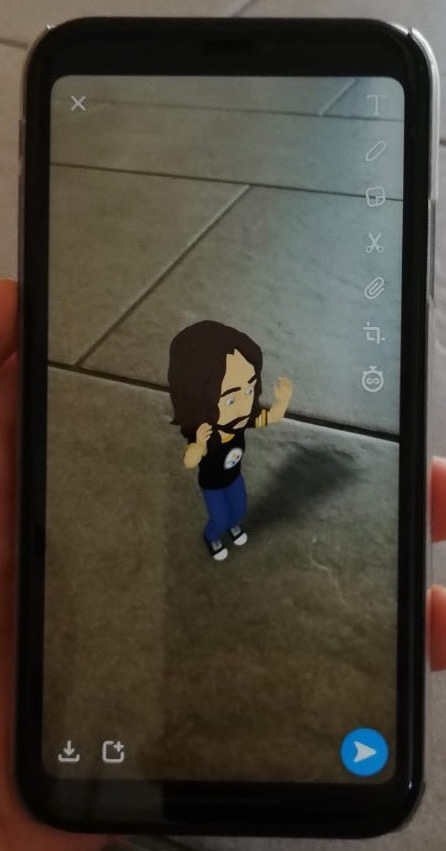
\includegraphics[width=10cm,height=7.5cm,keepaspectratio]{2Grundlagen/Bilder/snapchatAR.jpeg}
    \caption{Mobile-AR in Snapchat}
    \label{pic:snapchatAR}
\end{figure}
\subsection*{Smart-Brillen AR}
Unter Smart- oder Datenbrillen und Smart Glasses wird ein Konstrukt verstanden, das eine Brille mit einem tragbaren Minicomputer verwirklicht. 
Dabei werden Informationen über kleinste Monitore oder Prismen ausgegeben und dem Nutzer zusätzlich in das Sichtfeld projiziert. Im Gegensatz
zur mobilen \acs{AR} hat der Nutzer kein Gerät in der Hand und ist somit in seiner Bewegung weniger eingeschränkt und flexibler. 
\\ 
\linebreak
Die Technologie der Smart-Brillen ist ein ähnliches Konzept zu der \acs{VR}-Brille, allerdings befindet sich die Smart-Brille für den 
öffentlichen Gebrauch noch in der Entwicklungsphase, da nur bedingte Funktionen möglich sind und die Kosten für den Normalverbraucher nur 
bedingt tragbar erscheinen. Mit der überarbeiteten Version der \textit{HoloLens 2} von Microsoft ist eine deutlich komfortablere 
Möglichkeiten des alltäglichen Gebrauchs geboten, da diese im Vergleich zum Vorgängermodell deutlich komfortabler, leichter und 
handlicher ist. Das Design der Datenbrille ist von einer normalen Brille noch weit entfernt, ermöglicht mittlerweile aber das 
uneingeschränkte Sehen und Wahrnehmen der Umgebung. Die Bedienung des Geräts basiert auf schon vorhandenen Möglichkeiten die bereits in anderen 
Geräten Anwendung finden. Darunter gibt es am Gerät angebrachte Touchsensoren, Handbewegungen und -gesten und Eye-Tracking. 
\begin{figure}[hbt!]
    \centering
    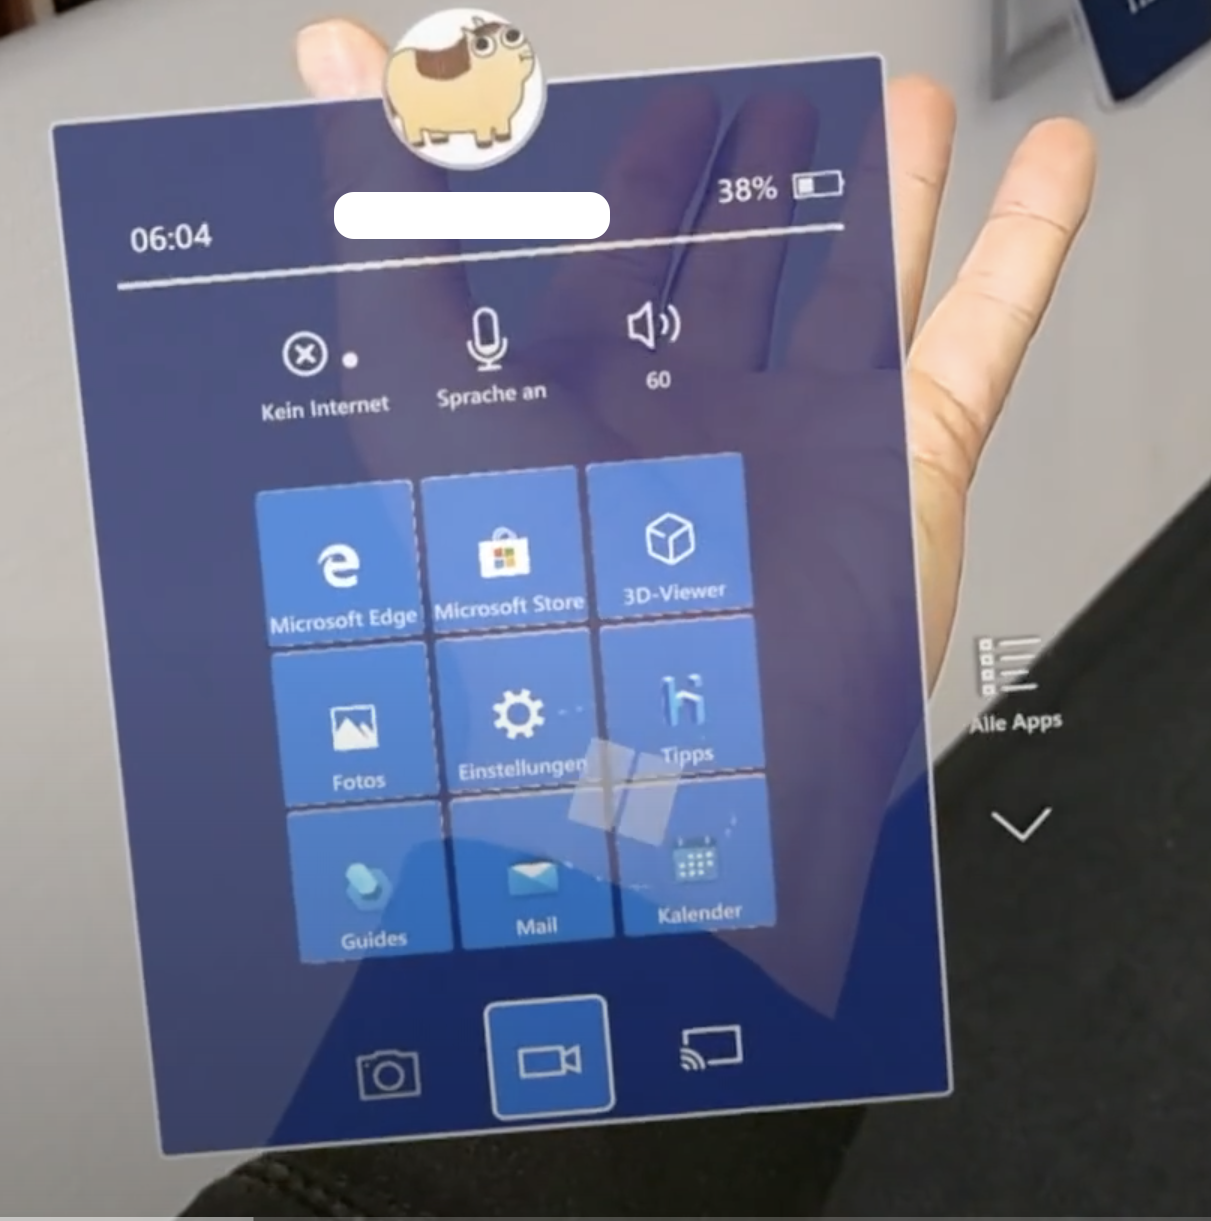
\includegraphics[width=10cm,height=7.5cm,keepaspectratio]{2Grundlagen/Bilder/smartglassAW.png}
    \caption{Test der HoloLens 2}
    \label{pic:testholo}
\end{figure}
\\ 
\linebreak 
Speziell im industriellen Bezug bieten die neuentwickelten Brillen ein komfortables und akzeptables Gewicht, sodass diese ohne große 
Probleme dauerhaft tragbar sind und den Mitarbeiter bei seiner Arbeit nicht übermäßig einschränken.
\\ 
\linebreak
Die Programmierung solcher \acs{AR}-Brillen laufen häufig über eigene \acs{SDK}s und plattformunabhängige Laufzeit- und 
Entwicklungsumgebungen, z.B. Unity oder Unreal Engine. Diese gelten als führende Produkte im Bereich der 3D-Echtzeitdarstellung.
Ein marktführendes Produkt ist unter anderem die Microsoft HoloLens 2, die der folgenden Abbildung zu entnehmen ist. 
\begin{figure}[hbt!]
    \centering
    \subfigure[Google Glass 2]{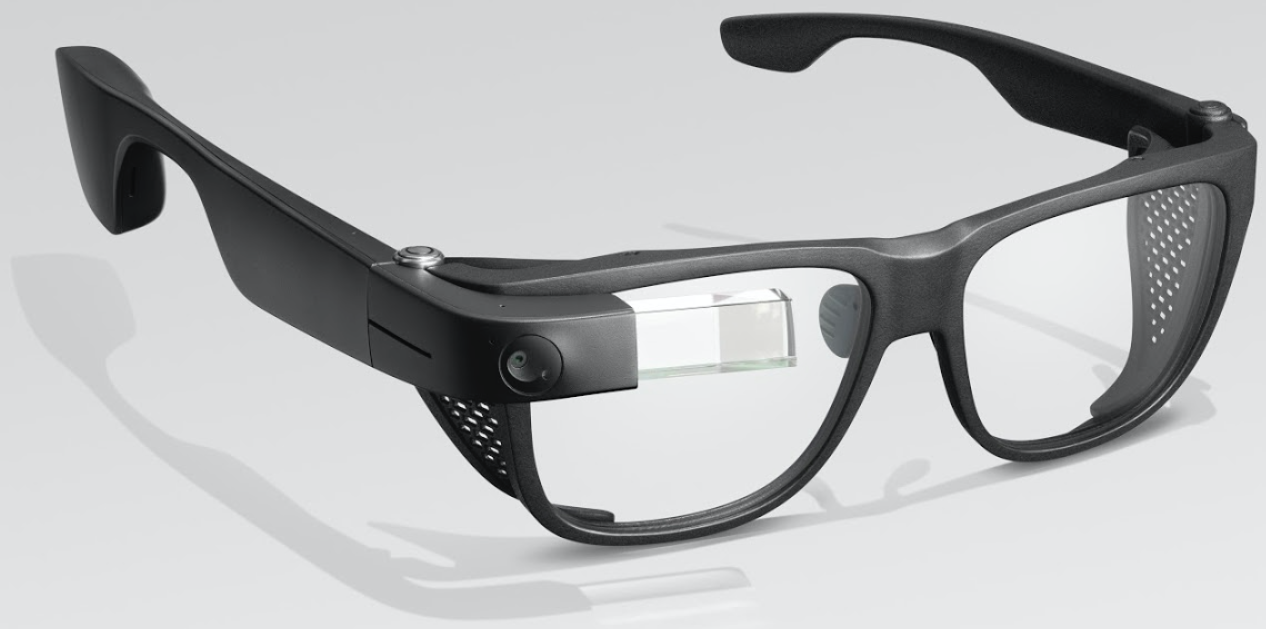
\includegraphics[width=7.5cm,height=5cm,keepaspectratio]{2Grundlagen/Bilder/googleglass.png}}
    \subfigure[HoloLens 2]{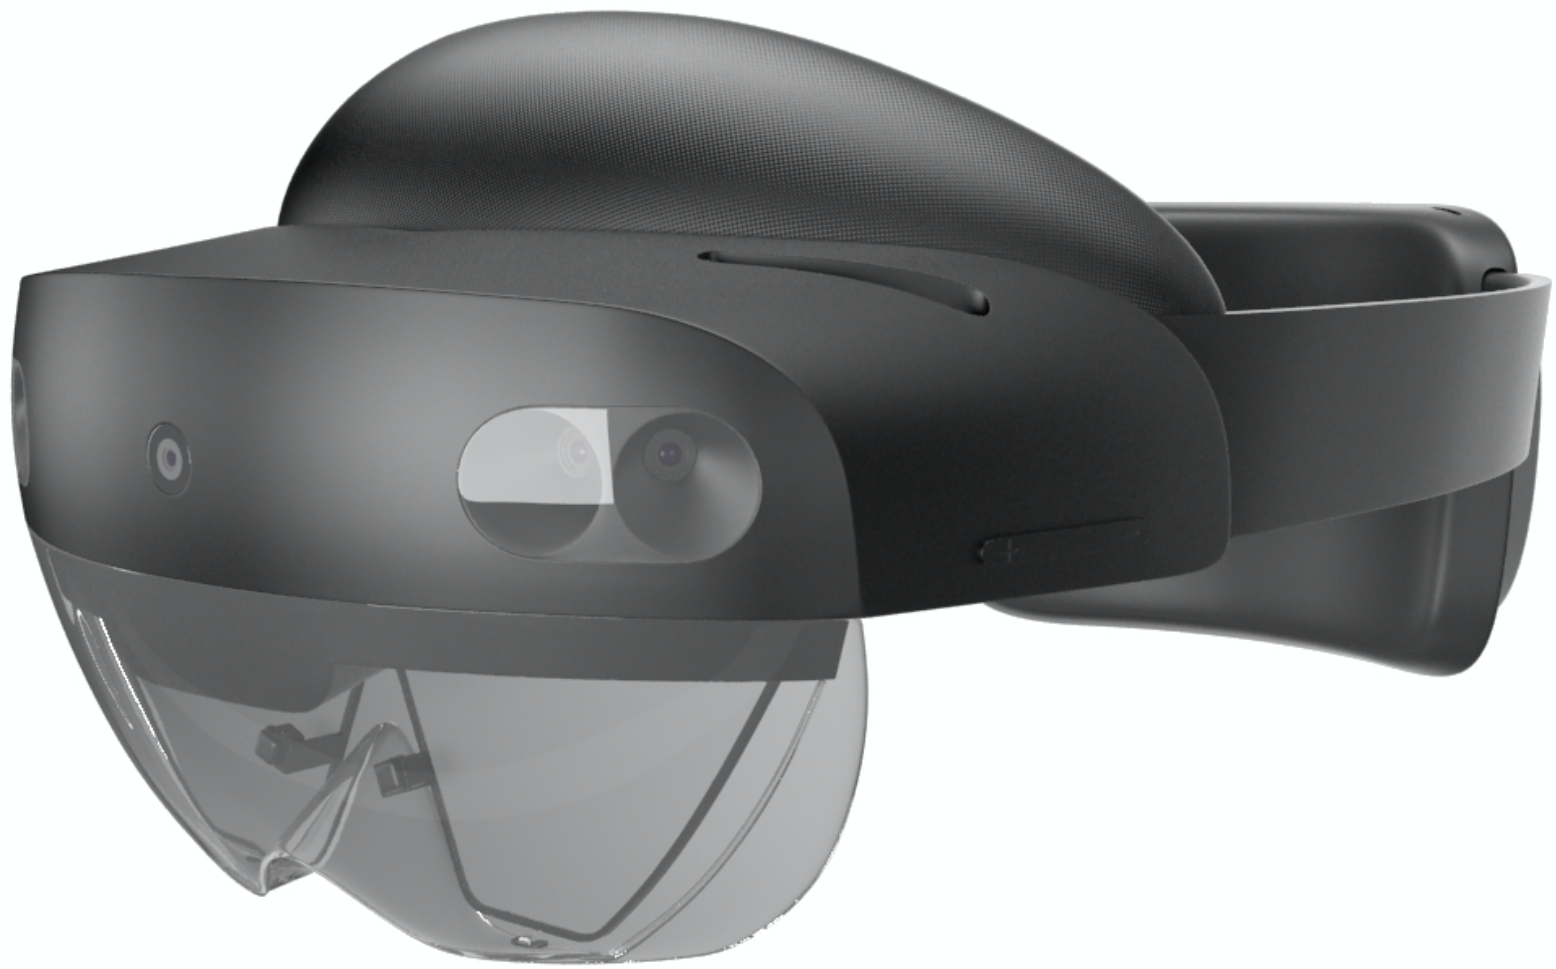
\includegraphics[width=7.5cm,height=5cm,keepaspectratio]{2Grundlagen/Bilder/hololensside.png}}
    \caption{Datenbrillen (\acs{HMD})}
    \label{pic:datenbrillen}
\end{figure}
\\ 
\linebreak
Eine schwer zu umgehende Herausforderung der \acl{AR} ist die Bestimmung der Position in der Daten und Objekte projiziert werden. Auf die 
Ansätze, diese Herausforderung zu bewältigen, wird in folgendem Abschnitt \ref{sec:posi} eingegangen.
\subsection{Positionsbestimmung}
\label{sec:posi}
Um ein digitales Objekt als Overlay dem Kamera-Live-Bild hinzuzufügen, werden genauestens definierte Positionen benötigt. Diese Positionen 
können durch unterschiedliche Ansätze ermittelt werden. Je nach Anwendungsfall, z.B. als Navigation, Routenplaner oder Google Maps 
\textit{„Live View“} \cite{googleliveview.2019a}, reicht eine etwas ungenauere Positionsbestimmung per \acs{GPS}, da in Relation zur 
realen Welt eine Abweichung um Zentimeter oder wenige Meter nicht von belangen ist. Bei Positionsbestimmungen auf kleinstem Raum ist eine 
genaue Lokation wichtig und basiert auf einem deutlich präziseren Ansatz. 
\\ 
Welche oben genannten Ansätze es gibt und welche Unterschiede zu beachten sind, wird in Folgendem näher darauf eingegangen. 
\subsubsection*{Marker-basierte Positionsbestimmung}
Speziell bei der Marker-basierten Positionsbestimmung gibt es verschiedene Möglichkeiten den Marker zu gestalten. Es können 
Binär- oder QR-Codes als Markierung verwendet werden, ein Beispiel eines solchen Codes ist der Abbildung \ref{pic:markerARpos} zu entnehmen. 
Diese Codes sind meistens quadratisch und haben ein eindeutiges Zeichen in der Mitte. Um die Rechenzeit gering zu halten gibt es einfache Muster, 
wie die Abbildung \ref{pic:markerARpos} zeigt.
\begin{figure}[hbt!]
    \centering
    
\includegraphics[width=5cm,height=5cm,keepaspectratio]{2Grundlagen/Bilder/bildmarkerAR.png}
    \caption{Marker-basierte Augmented Reality Positionsbestimmung}
    \label{pic:markerARpos}
\end{figure}
Neben der einfachen Markierungserkennung gibt es eine weiterentwickelte Möglichkeit der Bild- sowie der Objekterkennung. Diese sind Ansätze 
die grundlegend auf dem Ausgangspunkt des Binär-Code-Verfahrens aufbauen. Eine detailliertere Erläuterung der soeben genannten 
Erkennungsmöglichkeiten findet im Rahmen dieser Arbeit nicht statt. Allerdings wird allgemein kurz auf die Funktionsweise einer 
Marker-basierten Positionsbestimmung eingegangen.
\\ 
Durch ein Kamerabild wird nach einem vordefinierten Marker, bzw. nach einer festgelegten Markierung gesucht. Ist diese mit der Kamera erfasst, 
wird die Markierung durch Bildverarbeitungsalgorithmen und bestimmter Filterung eindeutig identifiziert. Mit den gewonnen Informationen und 
der Übereinstimmung des angegebenen Codes wird die Position, sowie die Orientierung des Markers berechnet. Mit den Angaben der Lage und 
Orientierung wird auf der Markierung das anzuzeigende digitale Objekt generiert und als Overlay über dem Kamerabild angezeigt. Die Markierung 
dient sozusagen als Grundlage um den digitalen Gegenstand überhaupt anzeigen zu können.
\\ 
Da der Marker immer im Blickfeld der Kamera sein muss, um das virtuelle Objekt anzuzeigen, bringt diese Art der Positionsbestimmung eine 
enorme Einschränkung mit sich, die in diesem Bezug unumgänglich ist. 
\\ 
\linebreak
Ein weiterer Ansatz der Positionsbestimmung ist als Überbegriff das Gegenstück zur oben aufgeführten Lokalisierung von Markern, die 
sogenannte Marker-unabhängige Positionsbestimmung, welche ebenso verschiedene Ausführungen vorweist. 
\subsubsection*{\acs{GPS}-basierte Positionsbestimmung}
Die Methode des \acs{GPS}-basierten Positionsbestimmungsverfahren verwendet hauptsächlich die Koordinaten der realen Welt. In Zusammenarbeit 
mit zusätzlichen im Anwendungsgerät verbauten internen Sensoren, bspw. Positions-, Geschwindigkeits- und Beschleunigungssensoren und Teile des 
\ac{INS}, z.B. dem Gyroskop, kann diese Art der Positionsbestimmung optimal Anwendung finden. Allerdings werden dabei deutlich mehr Komponenten
benötigt und ist deutlich komplexer umzusetzen, als ein markerbasiertes System. 
\\ 
Bei einem Anwendungsfall von \acs{GPS}-basierter Positionsbestimmung geht es meist um Routenplaner, Navigation oder Szenarien die sich 
auf offenen Flächen abspielen, da im Gegensatz zu Marker-basierten Anwendungen das Größenverhältnis deutlich geräumiger ist. Der Benutzer ist 
nicht auf einen bestimmten Bezirk beschränkt und ist nicht auf die millimetergenauer Darstellung angewiesen.
\\ 
\linebreak
Eine Alternative zu \acs{GPS} ist die Anwendung des \acs{SLAM}-Verfahrens. Dabei wird eine virtuelle Karte, bzw. ein geometrischen Modell der 
Umgebung erstellt. Wichtige Grundlagen zum Erzeugen eines solchen Modells sind eigenständig gefundene Landmarken die gleichzeitig 
lokalisiert werden. Darauf folgt ein Vergleich der Pose, der Position des Geräts und der geschätzten Karteninformationen aus dem Scan der 
Umgebung. 
Damit sind im erweiterten Sinne Marker geschaffen, die Anhaltspunkte für \acl{AR}-Interaktionen schaffen.
\\ 
In Kapitel \ref{chap:SLAM} wird die Thematik des \acs{SLAM}-Verfahrens genauestens erläutert. 

\subsection{Augmented Reality in der Industrie}
Das weit gefächerte Portfolio der \acl{AR} umfasst viele Anwendungsbereiche und Fachgebiete. Selbst dem übergeordneten Bereich der Industrie 
gibt es viele verschiedene Einsatzgebiete. Aus den vielen Möglichkeiten der Anwendung haben sich über die Jahre der Entwicklung der Technologie 
einige Gebiete in der Industrie herauskristallisiert, die besonders hohen Nutzen stiften. \cite{einsatzgebietear.2017a} In den Bereichen 
Instandhaltung und Wartung, Betrieb und Training ist \acl{AR} auf bestem Wege fester Bestandteil des Alltags zu werden. Bei dieser Betrachtung 
ist es sinnvoll sich auf die damit einhergehenden Lösungen zu fokussieren, die Reduktion der Kosten und dem Zeitaufwand, sowie die Verbesserung 
der Sicherheit. \cite{studieptc.2020j} 
\\ 
\linebreak
Bei einer Wartung oder Reparatur einer Maschine sind notwendige Informationen direkt greifbar und werden Schritt für Schritt angezeigt, sodass 
in bestimmten Situationen selbst ein Leihe die Anweisungen befolgen könnte. So werden zusätzliche Recherchearbeiten oder Unklarheiten über 
Vorgänge aus dem Weg geräumt. Ein Mitarbeiter kann so mit einem Tablet oder einer Smart-Glas Anweisungen visuell auf die realen Maschinen 
projizieren und Arbeitsschritte im Sichtfeld anzeigen lassen. Ebenso geht dieser Vorgang auch bei der Produktion von Bauteilen o.ä., indem 
eine \acs{AR}-Anwendung Anweisungen und Prozessschritte, z.B. auf das Werkstück oder Produkt, projiziert.
\\ 
Die Inbetriebnahme oder Bedienung einer komplexen Anlage oder Maschine ist nach herkömmlichen Standard enorm zeitintensiv und dadurch können
zusätzlich viele Fragen aufkommen, die meist den Prozess noch länger gestalten als vorgesehen. \acs{AR}-Anwendungen können 
Bedienungsanleitung oder -hilfen digitalisiert, indem Informationen, Inhalte oder Bedienelemente durch \acl{AR} auf der Anlage platziert werden. 
\\ 
In Fortbildungen, Schulungen oder Einarbeitungen in neue Geräte kann \acs{AR} durchaus von großem Vorteil sein. Mit wenig Aufwand, einem 
effektiveren Training können Schulungen interaktiver und vor allem sicherer abgehalten werden. Durch die Visualisierung der Trainings- und 
Schulungsinhalten verbessert sich der Lernprozess und damit wird auch die Nutzung der Maschinen verständlicher. \cite{einsatzgebietear.2017a}

\section{SLAM - Simultanious Localization And Mapping}
\label{chap:SLAM}
Als Simultaneous Localization and Mapping auch \acs{SLAM}-Problem gennant, bezeichnet man die Aufgabe, die Trajektorie \footnote{Lösungskurve oder Bewegungspfad eines Objekts} 
samt Orientierungsinformation einer sich bewegenden Plattform, z.B. ein Smartphone, Tablet oder jegliche Art von Roboter, aus 
Beobachtungen zu schätzen und gleichzeitig aus den gewonnenen Informationen eine Karte der Umgebung zu erstellen.
Diese Aufgabe ist für den weiteren Prozess von hoher Bedeutung. Zum einen sollen die generierten Karten sehr präzise sein, um einen hohen 
Wert für den Nutzer oder für spezielle Anwendungen, die auf der Karte aufbauen, darzustellen. Zum anderen benötigen autonome Roboter, 
beispielsweise Saug- oder Mähroboter, ein solch erzeugtes geometrisches Modell der Umgebung, um zielgerichtet selbstständig navigieren zu 
können. %\cite{slamdefi.2016a} 
\begin{quote}
    Das Simultaneous Localization and Mapping oder kurz SLAM Problem behandelt das gleichzeitige Schätzen der Position und Ausrichtung einer 
    mobilen Plattform im Raum anhand der sich an Bord befindlichen Sensoren sowie den Aufbau eines Modells der Umgebung. Dieses Problem ist 
    von großer praktischer Relevanz und ist Kernbestandteil der meisten mobilen Sensor- systeme. \cite{slamdefi.2016a}
\end{quote}
1986 wurden auf der \textit{IEEE Robotics and Automation Conference} erste mathematische Definitionen vorgenommen, die mittels statischer 
Theorien ermittelt und mit ersten Studien belegt wurden. Einige Jahre später,im Jahr 1995, wurde das \acs{SLAM} Problem erstmals auf dem 
internationalen Symposium für Robotikforschung (\textit{ISRR'95}) vorgestellt. Die Forschungen hielten an, bis auf der (\textit{ISRR'99}) 
die erste \acs{SLAM} Sitzung stattfand. 
\subsection{Definition des Problems}
Angenommen ein Roboter startet in einer Position auch Pose gennant und Konfiguration \textit{p0} und bewegt sich durch eine ihm 
unbekannte Umgebung, wobei diese nicht vorhandenen Kenntnise das Hauptproblem darstellen. Die Einstellung beinhaltet Position und Ausrichtung 
des Roboters. Je nach Bewegung in Raum oder Ebene ist die Pose meist als 3- oder 6-dimensionaler Vektor abgebildet. Die Bewegung des 
Roboters wird durch bekannte Kontrollkommandos \textit{u} angewiesen, allerdings mit einer gewissen Unsicherheit versehen. Dabei wird 
zwischen den Zeitpunkten \textit{t-1} und \textit{t} die Bewegung des Roboters mit \textit{ut} beschrieben und somit auch die 
unterschiedlichen Posen \textit{pt-1} nach \textit{pt}. Die Umgebung wird parallel dazu über diverse Sensoren, z.B. interne Sensoren, bspw. 
Gechwindigkeits- oder Positionssensoren, und externer Senoren, unter anderem Abstands- oder taktile Sensoren. Neben der Protokollierung der 
Position, bei der es zu Störungen oder Berechnungsfehler kommen kann, gibt es Beobachtungen durch Sensoren die verrauscht \textit{zt} sind.
\\ 
\linebreak
Mit diesen vorhandenen Werten ist das Ziel die Schätzung der Trajektorie \textit{p0:T=[p0,p1,...,pT]T} des Roboters von Beginn der 
Fortbewegung bis zum Zeitpunkt \textit{T}. Gleichzeitig zur Berechnung der Trajektorie wird eine Karte \textit{m} des Umfelds geschätzt, 
deren Darstellung den Anforderungen entsprechend angepasst werden kann. Mit den Anforderungen sind verschiedene Repräsentationen der Karten 
gemeint, darunter beispielsweise eine Veranschaulichung von Punktansammlungen an Gegenständen, gerenderte Oberflächenmodelle oder 
2D-Rasterkarten und verstärkt visualisierte 3D-Voxelkarten.\footnote{(Zusammensetzung aus dem englischen volume \textit{vox} und elements 
\textit{el}), bez. einen Gitterpunkt in einem dreidimensionalen Gitter.} Basierend auf den Sensormessintervallen \textit{z1:T} und den dabei
stattfindenden Kontrollkommandos \textit{u1:T} wird die Karte des Umfeldes und alle Positionen bestimmt. Die Wahrscheinlichkeitsverteilung 
\textit{p(p0:T,m|z1:T,u1:T)} wird durch die geschätzten Werte \textit{p0:T} und \textit{m} berechnet. 
\\ 
\linebreak
Die Berechnung der Wahrscheinlichkeitsverteilung ist auch unter dem Namen \textit{Offline-\acs{SLAM}} bekannt. In der Praxis ist allerdings 
die Schätzung der Position \textit{xt} und der Karte der Umgebung durch \textit{p(pt,m|z1:t,u1:t)} interessanter, da Roboter Entscheidungen 
basierend auf aktuellen Informationen, z.B. der Posenschätzung und dem Umgebungsmodell, treffen sollen. Die Variante der Echtzeitschätzung 
ist auch als \textit{Online-SLAM} bekannt. \cite{slamdefi.2016a}

\subsection{Localization}
Damit das Endgerät, Smartphone oder der Roboter seine Position in Erfahrung bringen und schätzen kann, werden Informationen und Möglichkeiten 
benötigt die Bewegung in irgendeiner Form zu messen. Da das Nutzergerät eine eigene virtuelle Karte, unabhängig von der \acs{GPS}-basierten 
Position, generiert, ist das \textit{Tracking} über die Weltkoordinaten nicht Bestandteil des eigentlichen Verfahrens. Für die Erfassung der 
internen Systemzustände gibt es sogenannte interne Sensoren die in dem Roboter zur Verfügung stehen. Bestandteile dieser internen 
Sensorik sind unter anderem Positions-, Geschwindigkeits-, Beschleunigungssensoren und das \acl{INS}. Für die Positions- und 
Geschwindigkeitserkennung gibt es z.B. einen optischen Codierer, welcher durch Lichtimpulse die Geschwindigkeit als auch die zurückgelegte 
Strecke schätzen kann. Das \acs{INS} besteht aus Lagesensoren und einem Kreiselkompass (Gyroskop), diese sind essentiell für die Bestimmung 
der Orientierung und Neigung des Geräts. Ausgehend von der Erdkugel beziehen sich diese Sensoren auf das gegebene inertiale Koordinatensystem.
\subsection{Mapping}
Um neben der Berechnung der Position durch die interne Sensorik die Umgebung registrieren und schätzen zu können, gibt es externe Sensoren 
die sich mit der Erfassung der Umwelt beschäftigen. Auch hier gibt es viele Arten von Sensoren mit denen es ermöglicht wird die Umgebung 
wahrzunehmen, darunter Taktile Sensoren, Näherungs-, Abstands-, Positionssensoren und Visuelle Sensoren. Hinsichtlich Abstandssensoren die 
Mesungen zwischen Gegenstand und Sensor durchführen, gibt es allgemein erhebliche Vorteile gegenüber den Näherungssensoren. Vorteile sind 
beispielsweise eine größere Reichweite und Blickfeld als Näherungssensoren, die Ermittlung der genauen Entfernung zu Gegenständen und sie 
sind besser zur Erfassung geometrischer Umweltinformationen geeignet. Für die Messung des Abstandes eignet sich die \ac{TOF}-Kamera, die 
mit dem Laufzeitverfahren Distanzen messen und berechnen kann. 
\\ 
Das Laufzeitverfahren funktioniert wie folgt:
\begin{align*}
    \textit{d} = \frac{1}{2}\textit{ct}
\end{align*}
Abstand zwischen der Zielfläche und dem Sensor \textit{d} ist das Produkt aus der Signalgeschwindigkeit \textit{c} und der messbaren Laufzeit 
\textit{t}. Beispiele für solche \acs{TOF}-Kameras und deren Repräsentation sind folgender Abbildung (\ref{pic:tofCam}) zu entnehmen.
\begin{figure}[hbt!]
    \centering
    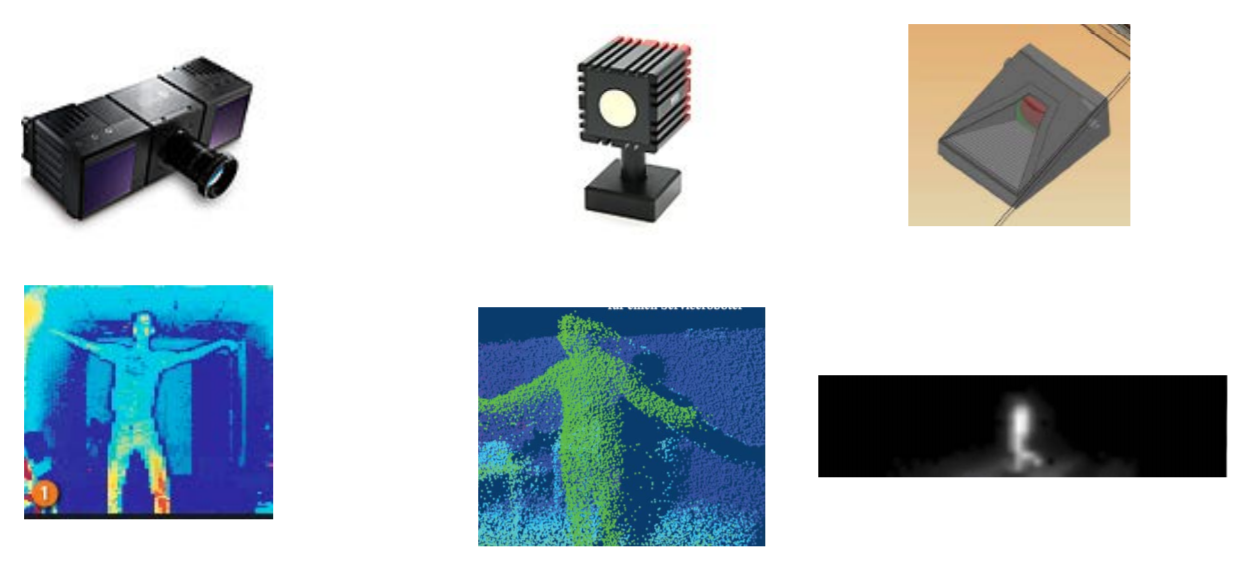
\includegraphics[width=13cm,height=13cm,keepaspectratio]{2Grundlagen/Bilder/tof_kamera.png}
    \caption{Time-of-Flight Kamera und deren Repräsentation \cite{robotik.2020m}}
    \label{pic:tofCam}
\end{figure}
\\ 
Auf der linken Seite ist eine PMD-Kamera zu sehen, gefolgt von einer SwissRanger-Kamera und auf der rechten Seite eine IFM-Kamera.
\subsection{Verfahren zur Lösung des SLAM Problems}
Das Lösen des \acs{SLAM}-Problems wird in der Praxis mit den angestellten Verfahren, die sich bei der Anwendung duchsetzten, durchgeführt. In 
folgenden Abschnitten werden zwei dieser Verfahren erläutert, sodass ein Grundverständnis vorhanden ist. Zuerst wird auf das Graph-basierte 
\acs{SLAM}, dem Lösen des Problems unter Anwendung der kleinsten-Quadrate Methode, eingegangen, darauffolgend die Lösung durch einen rekursiven 
Ansatz, dem erweiterten Kalman Filter (\acs{EKF}).

\section{Quaternionen}
\label{chap:Quaternionen}
%%%%%%%%%%%%%%%%%%%%%%%%%%%%%%%%%%%%%%%%%%%%
% -----------> tbd... !! <-----------------




%%%%%%%%%%%%%%%%%%%%%%%%%%%%%%%%

\subsection{Transformation}
\subsection{Rotation}


%%%%%%%%%%%%%%%%%%%%%%%%%%%%%%%%%%%%%%%%%%%%%%%%%%%%%%%%%%%%%%%%%%%%%%%%%%%%%
%% Descr:       Vorlage für Berichte der DHBW-Karlsruhe, Ein Kapitel
%% Author:      Prof. Dr. Jürgen Vollmer, vollmer@dhbw-karlsruhe.de
%% $Id: kapitel2.tex,v 1.5 2017/10/06 14:02:51 vollmer Exp $
%%  -*- coding: utf-8 -*-
%%%%%%%%%%%%%%%%%%%%%%%%%%%%%%%%%%%%%%%%%%%%%%%%%%%%%%%%%%%%%%%%%%%%%%%%%%%%%%%

\chapter{Technologien}
In diesem Kapitel werden alle für das Verständnis notwendigen und verwendeten Technologien aufgeführt und genauestens erläutert.
\\Die durch die Programmiersprache \textit{C\#}, von Microsoft, zur Verfügung gestellte Technologie \textit{WPF} wird in folgendem Auskunft über 
allgemeine Informationen, Funktionsweise, Einsatzgebiete und deren untergeordneten Technologien konkretisiert. 
\\Mit den vorab getätigten Überlegungen zu Zeichentechnologien die kompatibel mit \textit{C\#}, bzw. \textit{WPF} waren kam man zu der von Microsoft
entwickelten Zeichentool System.Drawing, die ebenso präzisiert wird.
%WPF: https://de.wikipedia.org/wiki/Windows_Presentation_Foundation am 08.04.2020, um 23:55 Uhr
%WPF: [WPF]https://docs.microsoft.com/de-de/dotnet/framework/wpf/getting-started/introduction-to-wpf-in-vs am 08.04.2020, um 23:55 Uhr
%WPF: https://www.wpf-tutorial.com/de/1/uber-wpf/was-ist-wpf/ am 08.04.2020, um 23:55 Uhr
%WPF: https://docs.microsoft.com/de-de/dotnet/framework/wpf/introduction-to-wpf am 08.04.2020, um 00:20 Uhr
\section{WPF (Mikka Jenne)}
\ac{WPF} in Visual Studio bietet Entwicklern ein einheitliches Programmiermodell zum 
Erstellen von Line-of-Business-Desktopanwendungen unter Windows. \cite{wpfmicrosoft.2020a} 
\\Das Grafik-Framework \acs{WPF}, sowie die Entwicklungsumgebung Visual Studio sind beides Produktionen des Unternehmens Microsoft.
Von Microsoft wird es als das Framework zur Erstellung von Desktop-Clientanwendungen für Windows mit visuell herausragenden 
Benutzerflächen umworben.
\linebreak
Der Kern von \textit{WPF} ist eine auflösungsunabhängige und vektorbasierte Rendering-Engine, die die Leistungsfähigkeit 
moderner Grafikhardware nutzt. [WPF Kern] Dieser Kern wird durch \textit{WPF} um mehrere Features zur Entwicklung von Anwendungen 
erweitert. Zu den Erweiterungen des \textit{WPF}-Kerns zählen unteranderem die Beschreibungssprache Extensible Application Markup Language \textit{XAML}, 
die in der nächsten Sektion konkretisiert wird, diverse Steuerelemente, Datenbindungen, 2D- und 3D-Grafik, Animationen, Vorlagen, Dokumente, Texte 
und Typographie.
\\Die Anlehnung von \textit{WPF} an \textit{.NET}-Typen ist sehr stark, da \textit{WPF} eine Teilmenge von \textit{.NET} ist. Die Typen von \textit{.NET} sind zum größten Teil im 
Namespace System.Windows, welcher im Nachgang noch genauer aufgezeigt wird, wiederzufinden. 
\\Das Grafik-Framework kann in zweierlei Programmiersprachen implementiert werden, zum einen unter der Nutzung von \textit{C\#} und zum anderen kann 
Visual Basic verwendet werden. 
\\Microsoft entwickelte viele Technologien und Frameworks, die die themenübergreifende Nutzung möglich machen, bzw. die Einfachheit besitzen 
durch die vorhandenen Grundlagen viele dieser Technologien nutzen zu können ohne neues Wissen aneignen zu müssen, da die Grundlagen identisch 
sind. Zu diesen Technologien gehören \textit{ASP.NET} und Windows Forms als Vorgänger von \textit{WPF}.
%Allgemein was das ist
%Wie es funktioniert, was es macht
%Welche Möglichkeiten es mit WPF gibt
%Welche verfügbaren Komponenten es dazu gibt (XAML, etc.) 
\subsection{XAML - Extensible Application Markup Language} % https://de.wikipedia.org/wiki/Extensible_Application_Markup_Language am 01.04.2020, um 18:00 Uhr
Allgemein ist \ac{XAML} eine Beschreibungssprache zur Gestaltung grafischer Benutzeroberflächen, entwickelt von Microsoft. Die neue deklarative 
Sprache wurde für das Framework \textit{.Net 3.0} in Windows Presentation Foundation \textit{WPF} für \textit{WPF}-Windows-Anwendungen entwickelt. \cite{wpf.2020a} 
\\Die Extensible Application Markup Language ist eine XML-basierende Sprache, die verwendet wird, um Benutzeroberflächen, Verhaltensweisen, 
Animationen, grafische Elemente etc. zu definieren. 
\subsection*{Window - Fenster}
Ein Code-Template eines standardmäßigen Fensters \textit{Window} sieht wie folgt aus und wird so als Basis-XAML zur Verfügung gestellt.
% \begin{figure}[hbt!]
    % \centering
    % 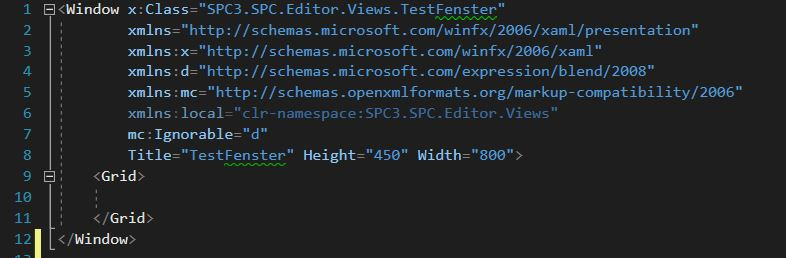
\includegraphics[width=15cm,height=10cm,keepaspectratio]{3Technologien/Bilder/XAML-CodeSnippet}
    % \caption{Window-Template}
% \end{figure}
\begin{lstlisting}[language=XML,
    frame=single,           % Ein Rahmen um den Code
    framexleftmargin=15pt,  % Rahmen link von den Zahlen
    style=algoBericht,
    label={window-template},
    captionpos=b,           % Caption unter den Code setzen
caption={Window-Template}]
<Window x:Class="WpfApplication1.Window1"
    xmlns="http://schemas.microsoft.com/winfx/2006/xaml/presentation"
    xmlns:x="http://schemas.microsoft.com/winfx/2006/xaml"
    Title="Window1" Height="300" Width="300">
    <Grid>

    </Grid>
</Window>
\end{lstlisting}
Der oben aufgeführte Ausschnitt zeigt eine \textit{XAML}-Datei, die ein vorgefertigtes Template von Microsoft darstellt. 
Bei Erstellung einer neuen Datei, bzw. einer Benutzeroberfläche, wird dieses Template zur Verfügung gestellt. Es
beinhaltet zu Anfang alle relevanten Informationen über Größe des Fensters und dessen Design. Ein Grid, 
welches ebenso in dem Template vorhanden ist, erfüllt die Funktion eines Koordinators. Das bedeutet, dass auf der 
Oberfläche ein Raster angelegt wird, welches die Positionen verschiedener Komponenten und Elementen koordiniert. So kann 
allen Elementen ein fester Platz, an dem es angeordnet sein soll, zugewiesen werden.
\linebreak
Ebenso umfasst ein \textit{Window} einen hypothetischen Container, bzw. ein Grundgerüst, welches als Repräsentation 
verschiedener Seiten \textit{Page} verwendet wird. Die Basisklasse stellt einen Standardrahmen, sowie eine Titelzeile, einem 
Maximierungs-, Minimierungs- und Schließknopf zur Verfügung.
\subsection*{Page - Seite}
Neben dem Template für ein Fenster gibt es anderweitige Templates, um das Erscheinungsbild von Oberflächen zu gestalten.
Zum Beispiel gibt es, wie im Absatz darüber erwähnt, die sogenannten Pages, die im Template sichtlich das Markup \textit{Window} 
durch \textit{Page} ersetzen. Der Funktionsunterschied is jedoch enorm, wogegen das Window ein Grundgerüst mitliefert, zeigt die 
Seite nur die Oberfläche ohne Rahmen, die verwendet werden kann.
% \begin{figure}[hbt!]
    % \centering
    % 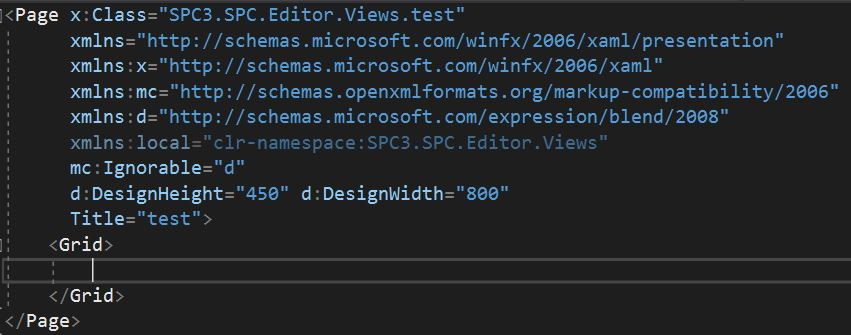
\includegraphics[width=15cm,height=10cm,keepaspectratio]{3Technologien/Bilder/PageXAML}
    % \caption{Page-Template}
% \end{figure}
\pagebreak
\begin{lstlisting}[language=XML,
    frame=single,           % Ein Rahmen um den Code
    framexleftmargin=15pt,  % Rahmen link von den Zahlen
    style=algoBericht,
    label={page-template},
    captionpos=b,           % Caption unter den Code setzen
caption={Page-Template}]
<Page x:Class="WpfApplication1.Page1"
    xmlns="http://schemas.microsoft.com/winfx/2006/xaml/presentation"
    xmlns:x="http://schemas.microsoft.com/winfx/2006/xaml"
    Title="Page1" Height="300" Width="300">
    <Grid>

    </Grid>
</Page>
\end{lstlisting}
\subsection*{UserControl - Benutzersteuerelement}
Eine dritte From der Repräsentation ist das sogenannte \textit{UserControl} (dt. Benutzerkontrolle), welches im Prinzip eine 
Mischung aus einem Window und einer Seite ist. Der Unterschied zwischen den einzelnen Elementen ist lediglich das Markup,
bzw. die Namensgebung \textit{UserControl}. 
\begin{lstlisting}[language=XML,
    frame=single,           % Ein Rahmen um den Code
    framexleftmargin=15pt,  % Rahmen link von den Zahlen
    style=algoBericht,
    label={usercontrol-template},
    captionpos=b,           % Caption unter den Code setzen
caption={UserControl-Template}]
<UserControl x:Class="WpfApplication1.UserControl1"
    xmlns="http://schemas.microsoft.com/winfx/2006/xaml/presentation"
    xmlns:x="http://schemas.microsoft.com/winfx/2006/xaml"
    Title="UserControl1" Height="300" Width="300">
    <Grid>

    </Grid>
</UserControl>
\end{lstlisting}
% https://www.c-sharpcorner.com/UploadFile/1e050f/grid-layout-in-wpf/ 
\subsection*{Grid}
Ein Grid ist ein Rasterelement in \textit{WPF} und teilt eine Seite oder ein Fenster in eine vorab definierte Anzahl von Zeilen und Spalten.
Das Raster ist ein sehr leistungsfähiges und nützliches Layout in WPF. 
Damit können untergeordnete Elemente in Zellen angeordnet werden, die durch Zeilen und Spalten definiert sind. 
Wenn ein neues XAML-Dokument erstellt wird, fügt Visual Studio automatisch ein Raster als ersten Container innerhalb des 
Fensterelements hinzu. Dieses vorgegebene Template kann durch \textit{Grid.ColumnDefinitions} in Spalten und durch \textit{Grid.RowDefinitions} 
in Zeilen unterteilt werden, wie dem folgenden Code-Ausschnitt zu entnehmen ist. \cite{wpftutorial.2020a}
\begin{lstlisting}[language=XML,
    frame=single,           % Ein Rahmen um den Code
    framexleftmargin=15pt,  % Rahmen link von den Zahlen
    style=algoBericht,
    label={gridtemplate},
    captionpos=b,           % Caption unter den Code setzen
caption={Grid-Template}]
<Grid.ColumnDefinitions>
	<ColumnDefinition/>
	<ColumnDefinition/>
</Grid.ColumnDefinitions>
<Grid.RowDefinitions>
	<RowDefinition />
	<RowDefinition />
</Grid.RowDefinitions>
\end{lstlisting}
% \begin{figure}[hbt!]
    % \centering
    % 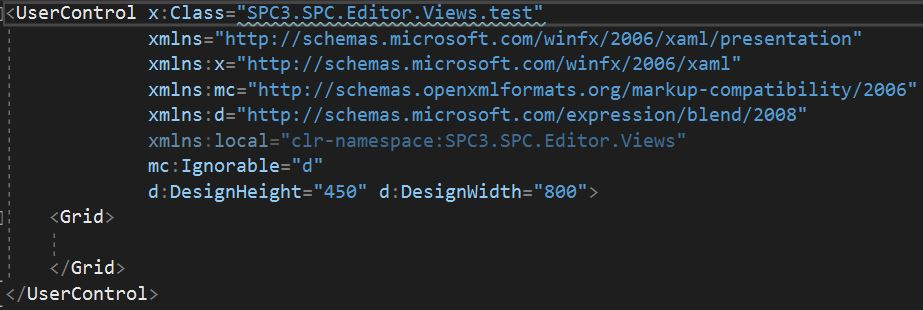
\includegraphics[width=15cm,height=10cm,keepaspectratio]{3Technologien/Bilder/UCXAML}
    % \caption{UserControl-Template}
% \end{figure}

% https://docs.microsoft.com/de-de/dotnet/api/system.windows?view=netcore-3.1 
\subsection{System.Windows}
\textit{System.Windows} ist ein in WPF deklarierter Namespace. Eine Bibliothek die viele essentiellen Methoden, verschiedene Klassen und 
WPF-Basiselementklassen zur Verfügung stellt. \cite{wpfmicrosoftwindow.2020a}
die das WPF-Eigenschaftensystem 
und die zugehörige Ereignislogik unterstützen, sowie andere Typen bereit, die häufig vom WPF-Kern und -Framework benötigt werden.
Die API, engl. Application Programming Interface, stellt zum Beispiel eine Drag \& Drop - Funktion bereit, die Hilfsmethoden und Felder für die Einleitung 
von Drag \& Drop-Vorgängen bietet. Zusätzlich beinhaltet diese Schnittstelle eine Methode zum Starten eines solchen Vorgangs und verwaltet 
und überwacht das Hinzufügen und Entfernen von Drag \& Drop-bezogenen Ereignishandlern.
\\Darüberhinaus gibt es viele weitere Methoden die über diesen Namespace zur Verfügung gestellt werden. 
\\Ein weiterer Namespace der in der Entwicklung verwendet wurde ist der sogenannte \textit{System.Collections}-Namespace, der in folgendem 
kurz beschrieben und mit einem Beispiel dargelegt wird.
% https://docs.microsoft.com/de-de/dotnet/api/system.collections?view=netcore-3.1
\subsection{System.Collections}
Der \textit{System.Collections}-Namespace enthält Schnittstellen und Klassen, die verschiedene Auflistungen von Objekten definieren, 
z.B. \textit{Listen}, \textit{Warteschlangen}, \textit{Bitarrays}, \textit{Hashtabellen} und Wörterbücher. \cite{wpfmicrosoftcollection.2020a}
Ein bekannter Parameter dieser Schnittstelle ist die \textit{ArrayList}, eine Anreihung von Feldern, die nach Anforderungen, bzw. nach Gebrauch
beliebig erweitert werden kann und Datenstrukturen der gleichen Form speichert.
\\Zur Implementierung der Hauptanwendung, das Zeichnen der Schaltpläne, werden die Schnittstellen des 
\textit{System.Drawings}-Namespaces verwendet.  

% https://docs.microsoft.com/de-de/dotnet/api/system.drawing?view=dotnet-plat-ext-3.1#classes 
\subsection{System.Drawing}
Der \textit{System.Drawing}-Namespace ist für die Darstellung von bestimmten Textformaten, Anzeigen von Graphiken 
durch \textit{Bitmaps} oder \textit{Icons} und ermöglicht den Zugriff auf die grundlegensten Grafikfunktionen. \cite{wpfmicrosoftdrawing.2020a} Durch weitere Namepsaces können diese 
Funktionen erweitert, bzw. verfeinert werden. Es werden über diesen Namespace auch Methoden zur händischen Zeichnung 
von Graphiken angeboten. 

\section{MVVM (Simon Leitl)}
\label{chap:MVVM}

Model-View-ViewModel ist ein Architekturmuster welches Entwicklern als Vorlage dient und hilft grafische Oberflächen standardisiert und strukturiert zu entwickeln. MVVM wird als Weiterentwicklung bekannter Architekturmuster wie MVC betrachtet. MVVM ist 2005 im Zuge der Entwicklung von WPF entstanden und ist mittlerweile bestandteil von Universal Apps und Webframeworks. MVVM trennt die Benutzeroberflächen von der Logik. Dabei wird die Logik in sogenannten ViewModel Klassen dargestellt. Die Benutzeroberfläche bindet sich an die Properties der ViewModel Klassen und erhält fast keinen prozeduralen Code. Setzt man das MVVM Pattern richtig um, enthalten die ViewModel Klassen keine Benutzeroberflächen Elemente. Dies ist ein großer Vorteil für das durchführen von Unit Tests. Die ViewModel Klasse selbst stellt öffentliche Properties und Commands zur Verfügung, an welche sich die View binden kann. Die Ebenen sind in \ref{pic:mvvm-pattern} zu sehen.
\begin{figure}[ht]
    \centering
    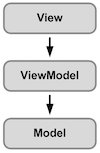
\includegraphics{3Technologien/Bilder/mvvmpattern}
    \caption{MVVM Pattern}
    \label{pic:mvvm-pattern}
\end{figure}
\linebreak
\\Die View Ebene wird zum Darstellen genutzt, die ViewModel Ebene enthält die Logik durch Commands und zuletzt das Model, welches die Daten enthält. 
\\Die Kommunikation zwischen der Benutzeroberfläche und der Logik wird durch sogenannte Bindings durchgeführt. Dabei werden Bestandteile der Benutzeroberfläche an das ViewModel oder bestimmte Commands des ViewModel, also der Logik gebindet. Über das Binding verläuft dann die Kommunikation zwischen den Komponenten. Dabei muss das Binding in der XAML Datei der View, einem Objekt zugewiesen werden, wie in Code-Beispiel ~\ref{xaml-binding} zu sehen ist. Die Zuweisung ist der Name einer Funktion, die im ViewModel vorhanden ist.
\\
\begin{lstlisting}[language=XML,
    frame=single,           % Ein Rahmen um den Code
    framexleftmargin=15pt,  % Rahmen link von den Zahlen
    style=algoBericht,
    label={xaml-binding},
    captionpos=b,           % Caption unter den Code setzen
caption={Binding in XAML}]
    <TextBlock Margin="3" Text="{Binding ViewModelNameList}"/>
\end{lstlisting}
Die Funktion wird dabei dem TextBlock aus dem Code-Beispiel ~\ref{xaml-binding} als Quelle zugewiesen. Über diese Funktion werden nun die Daten, die innerhalb des Textblocks auf der Oberfläche angezeigt werden, bezogen. Um die Daten im ViewModel entsprechend zur Verfügung zu stellen, wird eine Funktion benötigt. Diese Funktion besitzt einen Getter Methode, um die Daten über einen return auszugeben. Im Code-Beispiel \ref{viewmodel-binding} wird diese Funktion dargestellt. Sie enthält eine Liste in der die Namen aller VieModels gespeichert ist. 
\\
\begin{lstlisting}[language=C,
    frame=single,           % Ein Rahmen um den Code
    framexleftmargin=15pt,  % Rahmen link von den Zahlen
    style=algoBericht,
    label={viewmodel-binding},
    captionpos=b,           % Caption unter den Code setzen
    caption={Binding im ViewModel}]
public ObservableCollection<String> ViewModelNameList
{
    get { return _viewModelNameList; }
}
\end{lstlisting}
Die Funktion gibt die Namen eines ViewModel als String zurück. Dieser String wird dann innerhalb der TextBox in \ref{xaml-binding} abgebildet.
\\ Alle ViewModel die Funktionen für Bindings enthalten erben von der ViewModelBase Klasse. Dadurch wird die, in der ViewModelBase enthaltene \textit{INotifyPropertyChanged} Funktion implementiert. Diese ist Notwendig um Anzeigen auf der Oberfläche während der Laufzeit der Anwendung zu ändern und zu aktualisieren. 
Durch die \textit{INotifyPropertyChanged} erkennt die Anwendung zur Laufzeit Änderungen an der Oberfläche oder der Logik. Findet eine Änderung statt so ist die Funktion dafür verantwortlich, alle Teilnehmer des Bindings zu informieren und die Änderungen zu aktualisieren. \cite{mvvm.2010s}

\subsection{MVVM Light Framework}
MVVM Light ist ein Framework, das dazu entwickelt wurde MVVM Architekturen in Windows Universal, WPF, Silverlight, Xamarin.iOS, Xamarin.Android und Xamarin.Forms zu entwickeln. Dabei hilft das Framework bei der Erstellung der Strukturen innerhalb eines Projekts. Somit haben die Entwickler eine Basis, auf die sie sich bei der Umsetzung beziehen können. Dadurch erhält die Anwendung eine einfache und saubere Wartbarkeit sowie eine einfache Erweiterbarkeit. MVVM Light hilft dabei, die View vom Model zu trennen. Ein weiterer Vorteil des Frameworks sind die verbesserten Testmöglichkeiketen für das entwickelte Projekt. Es erstellt testbare Anwendungen welche über eine dünnere Benutzeroberfläche verfügen. \cite{mvvmLight.2020a}

\endinput
%%%%%%%%%%%%%%%%%%%%%%%%%%%%%%%%%%%%%%%%%%%%%%%%%%%%%%%%%%%%%%%%%%%%%%%%%%%%%%%


%%%%%%%%%%%%%%%%%%%%%%%%%%%%%%%%%%%%%%%%%%%%%%%%%%%%%%%%%%%%%%%%%%%%%%%%%%%%%
%% Descr:       Vorlage für Berichte der DHBW-Karlsruhe, Ein Kapitel
%% Author:      Prof. Dr. Jürgen Vollmer, vollmer@dhbw-karlsruhe.de
%% $Id: kapitel2.tex,v 1.5 2017/10/06 14:02:51 vollmer Exp $
%%  -*- coding: utf-8 -*-
%%%%%%%%%%%%%%%%%%%%%%%%%%%%%%%%%%%%%%%%%%%%%%%%%%%%%%%%%%%%%%%%%%%%%%%%%%%%%%%

\chapter{Systementwurf}
Dieses Kapitel widmet sich dem Systementwurf mit Bezug auf die in Kapitel 1 dargelegte Aufgabenstellung. Dabei wird die Softwarekonzeption 
dargestellt und Gründe für die Wahl der Frameworks genannt. 

\section{Architekturkonzept (Simon Leitl)}
Um Schaltpläne in der Gebäudetechnik, durch die Software zu realisieren, muss ein geeignetes Konzept, sowie ein erster Entwurf erstellt 
werden. Dieser wird als Basis für die künftigen Weiterentwicklungen verwendet. Die Anwendung muss in der Lage sein, auf Benutzerbedienungen 
zu reagieren, Skizzen zeichnen zu können und die Daten passend zu verändern. Wird ein Schaltplan gezeichnet, soll dieser gespeichert und bei 
der nächsten Ausführung wieder geöffnet werden können. Das ermöglicht die mehrmalige Anwendung des Systems für den Nutzer. 
\\Die entstehende Software soll für eine fortführende Entwicklung geeignet sein. Dafür wird ein modularer Aufbau vorgesehen. Dieser soll 
das einfache und schnelle Hinzufügen von Bestandteilen ermöglichen. Des weiteren besteht die Software aus verschiedenen Bestandteilen, die 
oft einzeln behandelt werden. Durch einen modularen Aufbau wird gewährleistet, dass die Module unabhängig voneinander bearbeitet und 
verändert werden können. Ein weiterer Faktor der Systemarchitektur ist das Verhältnis zwischen FrontEnd und BackEnd. Also dem View und der 
Logik. Für eine parallele Entwicklung bietet sich die Entkopplung zwischen der Benutzeroberfläche und der Logik an. Dies hat außerdem den 
Vorteil, dass bei späteren Änderungen der Benutzeroberfläche die Logik nicht angepasst werden muss. Für die entstehende Software wird sowohl 
eine Benutzeroberfläche, sowie eine Datenhaltung und systemweite Verarbeitungsprozesse benötigt. Da als Basissystem \textit{C\#} und das WPF Framework 
benutzt werden, wird für die Architektur das Model-View-ViewModel Pattern ausgewählt. Dieses begünstigt außerdem das Testen der Entwicklung. 
Durch MVVM können UI und BackEnd unabhängig voneinander getestet werden.
\\
Die Software wurde zunächst in zwei große Bausteine geteilt.
\begin{itemize}
    \item Startmenu
    \item Editor
\end{itemize} 
Neben den zwei Bausteinen, verfügt die Anwendung noch über zwei Ordnerstrukturen. Eine für das Speichern von Projekten, die andere für 
die Komponenten, die in das System geladen werden. Die Anwendung im gesamten Überblick ist in Abbildung \ref{pic:softwarearchitektur} 
sichtbar.
\\
\begin{figure}[hbt!]
    \centering
    \includegraphics{4Systementwurf/Bilder/softwarearchitektur}
    \caption{Software-Architektur}
    \label{pic:softwarearchitektur}
\end{figure}
\newpage
\subsection{Startmenü}
Der erste Baustein ist der Einstieg der Anwendung für den Nutzer. Hier wird die Möglichkeit geboten, neue Projekte anzulegen oder bestehende 
Projekte zu öffnen. Dieser soll immer beim Start der Anwendung erscheinen. Dem Nutzer sollen die Optionen über große Schaltflächen auf der 
Benutzeroberfläche zur Verfügung stehen. Das Startmenu zählt daher im ganzen als ein Modul der Software. Der Aufbau des Moduls ist in 
Abbildung \ref{pic:klassendiagramStartmenu} genauer sichtbar. 
\\
\begin{figure}[hbt!]
    \centering
    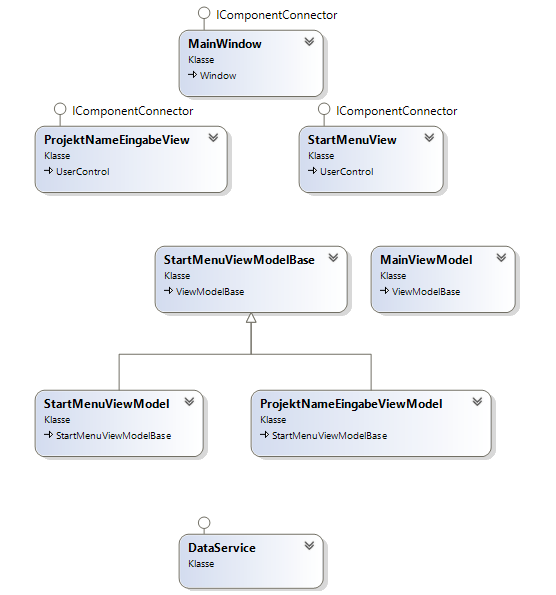
\includegraphics{4Systementwurf/Bilder/klassendiagramStartmenu}
    \caption{Klassendiagramm-Startmenü}
    \label{pic:klassendiagramStartmenu}
\end{figure}
\\ Die Klasse \textit{MainWindow} ist eine XAML Klasse und stellt somit eine Oberfläche dar. Sie bündelt die einzelnen Oberflächen des 
Startmenu. Beim Start der Anwendung öffnet das \textit{MainWindow} die erste Benutzeroberfläche der Software. Die Klasse selbst bindet 
die \textit{StartMenuView.XAML} ein. Diese ist, wie in Abbildung \ref{pic:klassendiagramStartmenu} zu entnehmen, als UserControl angelegt. 
Dies fördert insbesondere den modularen Aufbau der Software. Wird in der zukünftigen Weiterentwicklung etwas an der Startmenu-Komponente 
geändert, so muss nicht das komplette Window verändert werden, sondern ausschließlich der UserControl des Startmenu. Nach MVVM Prinzip 
benötigt das Startmenu-Modul auch eine oder mehrere ViewModel-Klassen, welche die Logik enthalten. Das Startmenu enthält vier 
ViewModel-Klassen:
\begin{itemize}
    \item  \textit{StartMenuViewModelBase}
    \item  \textit{MainViewModel}
    \item \textit{StartMenuViewModel}
    \item \textit{ProjektNameEingabeViewModel}
\end{itemize}  
\textit{StartMenuViewModelBase} und \textit{MainViewModel} erben von der globalen ViewModelBase Klasse, welche bereits in Kapitel 
\ref{chap:MVVM} beschrieben wurden. Sie sind der zentrale Anhaltspunkt für die Logik und beinhalten die Funktionen, welche von der 
Benutzeroberfläche direkt gebindet werden. 
\\Neben den ViewModels, enthält das StartMenu natürlich auch noch ein Model. Dieses ist in Abbildung \ref{pic:klassendiagramStartmenu} 
als \textit{DataService} dargestellt. Die DataService Klasse kümmert sich um die Bereitstellung der Daten. Hier insbesondere um die 
Bereitstellung der vorhandenen Projektdateien, die aufgerufen und geladen werden können.
\\Die zweite Funktion des Startmenus beinhaltet das Erstellen eines neuen Projekts. Dafür dient das ProjektNameEingabeView UserControl. 
Hier hat der Benutzer die Möglichkeit, einen Namen für das neu angelegte Projekt zu definieren. Das Projekt wird dann dementsprechend, mit 
dem vom Benutzer definierten Namen, in einer Ordner-Struktur gespeichert. Mehr zum Ablauf der Speicherung, sowie der Ordner-Struktur ist in 
Kapitel \ref{chap:UseCase-Startmenu} beschrieben. Um das Erzeugen der Datei des neuen Projekts durchzuführen, ist das 
\textit{ProjektNameEingabeViewModel} zuständig. 
\subsection{Editor}
\label{chap:Editor}
Der Editor enthält die eigentlichen Kernfunktionen der Anwendung. Hier sollen die Schaltpläne entstehen. Er erscheint nach dem im Startmenu 
ein neues Projekt angelegt, oder ein bestehendes Projekt ausgewählt wurde. Der Editor stellt eine Zeichenfläche bereit, in der es ermöglicht 
wird Schaltpläne zu skizzieren. Dabei werden durch verschiedene Werkzeugleisten, einzelne Komponenten zur Auswahl gestellt. Diese sind 
Notwendig um einen Schaltplan zu erstellen. Das Editor Fenster selbst, besteht aus einzelnen UserControls, um künftige Änderungen an der 
Oberfläche zu gewährleisten, ohne das diese Änderungen an den restlichen Elementen auslösen. Auch im Editor wird wieder nach dem Schema des 
MVVM Patterns vorgegangen. Dabei wird für jeden einzelne Element der Oberfläche, welche in UserControls angelegt werden, eigene ViewModels 
sowie Models erstellt. Beispielsweise enthält der Editor ein UserControl, der Werkzeuge zum Zeichnen der Leitungen bereitstellt. Nach MVVM 
wurden hier die folgenden Klassen erzeugt:
\begin{itemize}
    \item \textit{LeitungenToolsView}  
    \item \textit{LeitungenToolsViewModel} 
    \item \textit{LeitungenToolsModel}
\end{itemize}
Der Editor umfasst 
Alle User Controls des Editors werden in Kapitel \ref{chap:Softwarekonzept} genauer beschrieben.
\subsection{Programmier Richtlinien}
Um eine Übersichtlichkeit innerhalb des Projekts zu schaffen, damit auch künftig Entwickler, Änderungen an der Anwendung vornehmen können, wurden zu Beginn einige Richtlinien für die Programmierung und den Programmierstil festgelegt. 
\begin{itemize}
    \item Klassen, Variablen und Funktionen sollen aussagekräftige Namen erhalten. Wenn Möglich sollen die Namen den Inhalt bzw die Funktion der Klasse, Variable und Funktion beschreiben. 
    \item Klassen, Variablen und Funktionen die unterschiedliche Inhalte und Funktionen beinhalten, dürfen keinen ähnlichen Namen enthalten. Die Namen sollen für die Entwickler eindeutig unterscheidbar sein. 
    \item Aufgrund der Benutzung des MVVM Patterns, sind für Bestandteile der Anwendung meist drei Klassen enthalten. \textit{View, ViewModel, Model}. Die zugehörigen Klassen erhalten den gleichen Namen und unterscheiden sich lediglich in der Endung. Z.b. \textit{StartMenuView, StartMenuViewModel, StartMenuModel}.
\end{itemize} 
Diese Richtlinien dienen als Leitfaden für Entwickler. Sie sind an das Konzept Clean-Code angelehnt. 
\subsection{Mockups (Mikka Jenne)}
% https://www.degruyter.com/downloadpdf/books/9783110443882/9783110443882-005/9783110443882-005.pdf[3]
% https://www.gruenderszene.de/lexikon/begriffe/user-experience?interstitial [2]
% Foliensatz Advanced Software Engineering Maurice Müller Usability & UX
Bei der Entwicklung des allgemeinen Architekturkonzepts wurden parallel dazu auch erste grafische Entwürfe für die Darstellung der Benutzeroberflächen erstellt.
Dabei wurden User-Experience und Usability Faktoren berücksichtigt. \cite{gruenderszene.2020m}
\\
Die \ac{UX} umfasst alle Berührpunkte eines Nutzers mit einem Produkt, 
Dienstleistung oder Service. Sie spiegelt Erfahrungen sowie auch Empfindungen und Gefühle einer Person während der Benutzung eines Produktes wieder. \cite{foliensatz.2020m}
\\Usability (dt. Gebrauchstauglichkeit), ist ein Teil der User-Experience der speziell auf die exakte Gebrauchstauglichkeit der Anwendung, Dienstleistung
o.ä. abzielt. Dabei zu beachtende Faktoren sind unter anderem der Aufgabe, der Problemlösung angemessen und z.B. verständliche Anweisungen. 
\linebreak
Die für uns wichtigsten Faktoren der User-Experience und Usability wurden aus einer Menge bestehender Merkmale selektiert und während des Designs berücksichtigt. Diese Aspekte werden in
folgender Auflistung erläutert. \cite{degruyter.2020m}
\\
\linebreak
\begin{itemize}
    % \item Durchschaubarkeit
    % \begin{itemize}
        % \item Erlernbarkeit, Lernförderlichkeit
        % \item Ist es einfach, die Bedienung des Produkts zu verstehen und zu erlernen? Quelle: ISO 9241 (Teil 110 – dort als Lernförderlichkeit bezeichnet).
    % \end{itemize}
    \item Effizienz
    \begin{itemize}
        \item Der Nutzer kann seine Ziele mit minimalem zeitlichem und physischem Aufwand
        erreichen. Das Produkt reagiert schnell auf Nutzereingaben. Das Design der
        Nutzerschnittstelle macht keine unnötigen Arbeitsschritte erforderlich. Quelle: ISO 9241
        (Teil 11) bzw. (Teil 110 – Aufgabenangemessenheit).
    \end{itemize}
    % \item Immersion
    % \begin{itemize}
        % \item Wenn der Nutzer sich mit dem Produkt beschäftigt, vergisst dieser die Zeit. Der
        % Nutzer kann völlig in der Beschäftigung mit dem Produkt versinken. Dieses
        % Qualitätskriterium ist insbesondere bei Spielen und anderen zur Unterhaltung dienenden
        % Produkten relevant.
    % \end{itemize}
    \item Intuitive Bedienung
    \begin{itemize}
        \item Kann der Nutzer die Benutzerschnittstelle mit seinen vorhandenen
        Fähigkeiten unmittelbar und ohne jegliche Einarbeitung oder Anleitung durch andere
        bedienen? Quelle: Mohs et al. (2006).
    \end{itemize}
   % \item Leichtigkeit 
    %\begin{itemize}
    %    \item Es ist für den Nutzer einfach seine Aufgaben mit dem Produkt zu erledigen. 
    %    Die Interaktion mit dem Produkt ist weder körperlich noch mental anstrengend. Quelle: Hart und Staveland (1988) NASA-TLX (Task Load Index).
    %\end{itemize}
    %\item Nützlichkeit
    %\begin{itemize}
    %    \item Die Benutzung des Produkts bringt Vorteile. 
    %    \item Z.B. Produktivität und Effizienz bei Prozessen.
    %\end{itemize}
    %\item Schönheit
    %\begin{itemize}
    %    \item Ästhetik
    %    \item Das Produkt ist schön und ansprechend gestaltet. Das Produkt macht auf den Nutzer einen ästhetischen Eindruck.
    %\end{itemize}
    %\item Steuerbarkeit  
    %\begin{itemize}
    %    \item Kontrollierbarkeit, Fehlertoleranz, Robustheit
    %    \item Das Produkt reagiert immer vorhersehbar und konsistent auf Nutzerinteraktionen. Der Nutzer hat stets die volle Kontrolle über das Produkt. Quelle: ISO 9241 (Teil 110).
    %\end{itemize}
    %\item Übersichtlichkeit  
    %\begin{itemize}
    %    \item Visuelle Komplexität
    %    \item Die Benutzerschnittstelle wirkt aufgeräumt und übersichtlich und hat eine geringe visuelle Komplexität. Der Nutzer findet sich schnell darin 
    %    zurecht. Quelle: Müller und Schrepp (2013).
    %\end{itemize}
    %\item Vertrauen 
    %\begin{itemize}
    %    \item Die Daten und Informationen, die der Nutzer bei der Interaktion mit dem
    %    Produkt eingibt, sind in sicheren Händen. Dies spielt natürlich vor allem bei Produkten eine
    %    Rolle, bei denen der Nutzer kritische Daten preisgibt, z.B. beim Einkaufen in Web-Shops
    %    oder Online-Banking. Quelle: Corritore et al. (2001).
    %\end{itemize}
    \item Vollständigkeit 
    \begin{itemize}
        \item Das Produkt bietet dem Nutzer alles, was er oder sie erwartet. Es fühlt sich
        vollständig an, auch wenn es nicht tatsächlich alles im konkreten Nutzungskontext
        Notwendige bieten sollte. Der Faktor Vollständigkeit bezieht sich somit mehr auf die
        wahrgenommene Vollständigkeit und weniger auf die Summe der aufgabenangemessenen
        Nutzungskontexte. 
    \end{itemize}
\end{itemize}
Anhand der aufgelisteten Faktoren und der 
Umschreibung des zu lösenden Problems der 
Schaltplanzeichnung sind die aufgeführten Abbildung
4.3 und Abbildung 4.4 entstanden, die es galt in der Implementierung möglichst abbildungsgetreu wiederzugeben.
\pagebreak
\begin{figure}[htb]
    \section*{Startmenü Mockup}
    \centering
    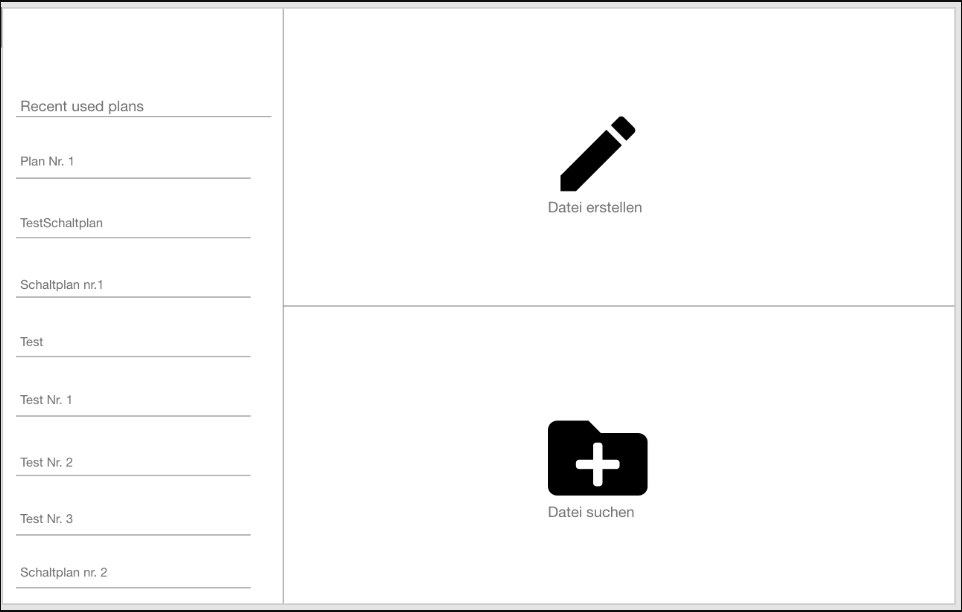
\includegraphics[width=15cm,height=10cm]{4Systementwurf/Bilder/StartMenuViewMockUp}
    \caption{Startmenü Mockup}
    \label{StartMenuViewMockUp}
\end{figure}
\\Die Benutzeroberfläche des Startmenüs ist einfach und selbsterklärend aufgebaut, sodass ohne große Worte der Umgang 
und der weitere Verlauf des Programms selbsterklärend ist. Die Oberfläche ist sichtlich in drei Rubriken eingeteilt, womit 
die wichtigsten Starteigenschaften 
repräsentiert werden.
\\
\linebreak
Über die in Abbildung 4.3 dargestellte Auflistung, getitelt mit \textit{Recent used plans}, werden alle erstellten Dokumente als Schnellzugriff zur
Verfügung gestellt. Jede einzelne Datei kann über diesen Menüpunkt aufgerufen und im Editor geöffnet werden. Zudem bietet diese Auflistung 
eine schnelle Übersicht über alle erstellten Dokumente. 
\\
\linebreak
Das rechte obere Drittel des Bildes stellt den Service zum Erstellen einer neuen Datei zur Verfügung. Durch klicken des Bildes, bzw. 
der Fläche wird das eigentliche Programm angestoßen, welches in dem Kapitel 5 Implementierung ausführlich erläutert und dargelegt wird.
\\
\linebreak
Das rechte untere Drittel weißt darauf hin einen Ordner öffnen zu können, damit vorhandene Dateien, 
z.B. aus anderen Ordnern, geöffnet und geladen werden können. Die genaue Vorgehensweise, bzw. die implementierten Funktionen
werden ebenso in Kapitel 5 genauestens dargestellt. 
\pagebreak
\\Ein simples Layout zum Start der Applikation, während die Editoransicht, der eigentliche Kern der Anwendung, deutlich 
mehr Funktionen und Möglichkeiten bietet.
Um die Abbildung 4.4 besser deuten zu können, wird nach Aufführung des Bildes eine Erklärung und eine kurze Begründung, wieso 
das Layout so gewählt wurde, stattfinden.
\\
\begin{figure}[htb]
   \section*{Editor Mockup}
   \centering
  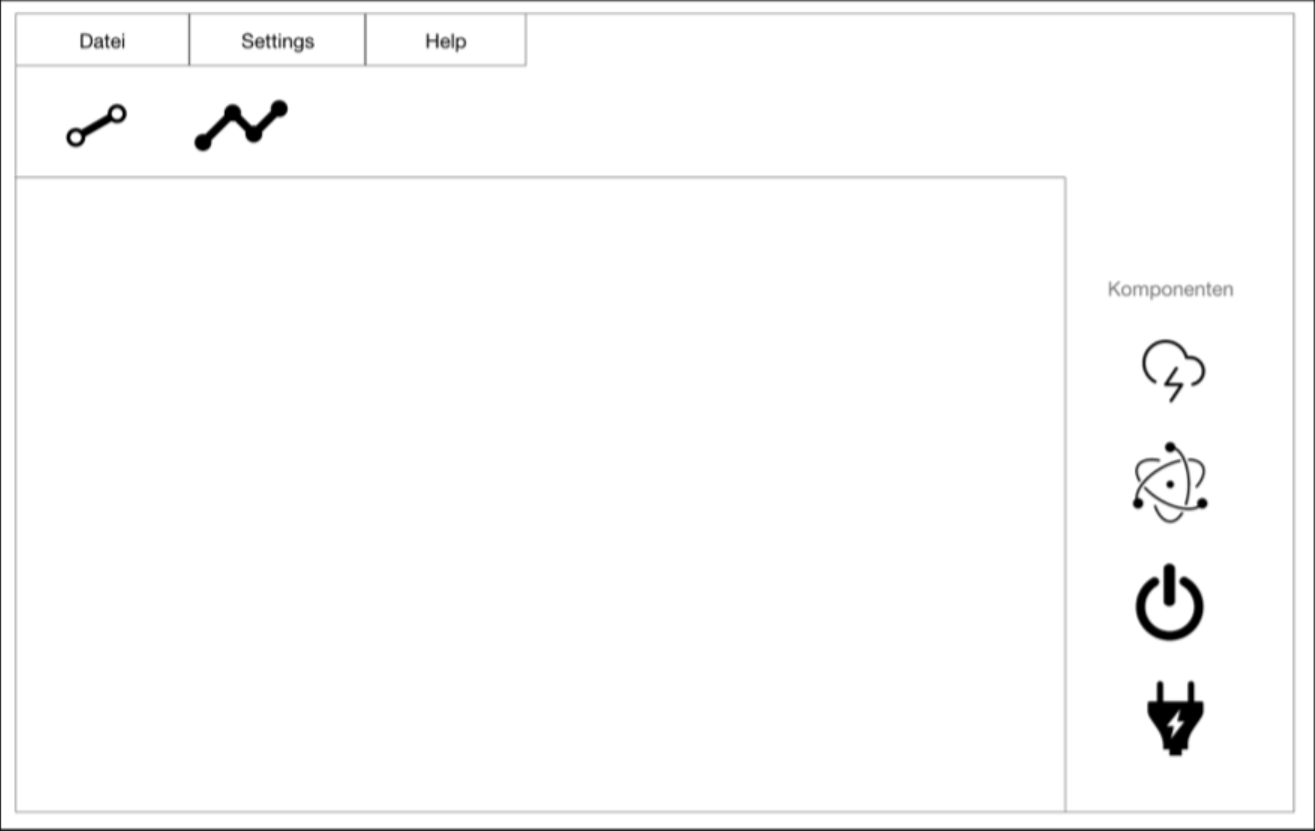
\includegraphics[width=15cm,height=10cm,keepaspectratio]{4Systementwurf/Bilder/EditorViewMockUp.png}
 \caption{Editor Mockup}
\end{figure} % https://www.wpftutorial.net/Canvas.html 
\\Wie in der Abbildung zu sehen ist, wird zentral eine weiße Fläche dargestellt. Diese Fläche repräsentiert ein Canvas, welches für die
Zeichnung der Schaltpläne geeignet ist. 
\\Das Canvas in WPF ist das grundlegendste Layout-Fenster für das Zeichnen von Objekten. Durch explizite Koordinaten können Elemente und 
Objekte in diesem Fenster positioniert werden. Die Koordinaten können relativ zu jeder Seite des Bedienfeldes im Canvas-Bereich angegeben 
werden.
\\
\linebreak
Die Oberfläche ist aufgeteilt in drei Segmente. Dies sind die Zeichenfläche als primäre Funktion, die zur Verfügung stehenden 
Komponenten zum Zeichnen angeordnet um das Canvas herum und die allgemeinen Einstellungen und Optionen als Reiterflächen im linken 
oberen Bereich. 
\\
\linebreak
Das entwickelte Design ist stark an andere bekannte Softwaredesigns, wie z.B. Microsoft Word, angelehnt, da dies ein gewohntes
Format ist und der Nutzer ungefähr, weiß wie das Programm zu benutzen ist, um schnell auf einen Fortschritt oder ein Ergebnis zu kommen. 
Trotz der Anlehnung an MS Word weicht es doch vom Design ab und kann damit nicht direkt und eindeutig verglichen werden. 
Vergleichbar sind z.B. die symbolisierten Flächen zum Auswählen verschiedenster Tools und Komponenten, die Einstellungsrubriken und 
die eigentliche Designfläche.
\section{Softwarekonzept (Simon Leitl)}
\label{chap:Softwarekonzept}
Im folgenden werden die einzelnen Bestandteile des in Kapitel \ref{chap:Editor} beschriebenes Editor, genauer erläutert. 
\begin{figure}[hbt!]
    \centering
    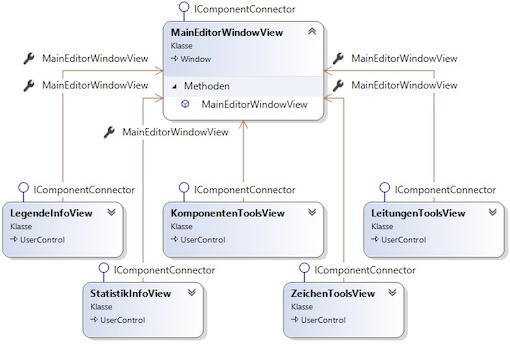
\includegraphics{4Systementwurf/Bilder/EditorView}
    \caption{Editor-viewKlassendiagramm}
    \label{pic:viewKlassendiagramm}
\end{figure}
\linebreak
Alle Bestandteile werden als UserControls in das MainEditorWindow eingebunden. Somit repräsentiert ein Fenster die verschiedenen Funktionen. Für die Implementierung sind diese jedoch abgekoppelte Bestandteile. Jedes UserControl kann einzeln und selbständig programmiert und gestaltet werden. Daher werden diese im Klassendiagramm (Abb. \ref{pic:viewKlassendiagramm}) als einzelne Klassen aufgeführt, mit Zuordnung zum MainEditorWindow. 
\subsection{Zeichenfläche}
Die Zeichenfläche ist der größte Bestandteil des Editors. Hier hat der Nutzer die Möglichkeit einen Schaltplan zu zeichnen. Dabei wählt er zunächst in den Werkzeugleisten ein Werkzeug aus. Wählt er beispielsweise ein Werkzeug zum zeichnen des Grundrisses aus den ZeichenTools aus, hat er die Möglichkeit innerhalb der Zeichenfläche einen Grundriss zu zeichnen. 
\subsection{KomponentenTools}
Die KomponentenTools sind eine Werkzeugleiste, welche dem Benutzer die für einen Schaltplan benötigten elektrischen Komponenten zur Verfügung stellt. Solche sind zum Beispiel eine Steckdose oder eine Leuchte. Die Komponenten verfügen über einen Namen sowie ein Symbol, um sie eindeutig zu identifizieren. Das Symbol einer Komponente wird später im Schaltplan angezeigt, sofern es benutzt wird.
\subsection{LeitungenTools}
Die LeitungenTools sind eine weitere Werkzeugleiste, welche dem Benutzer die für einen Schaltplan benötigten Leitungen zur Verfügung stellen. Hierbei gibts es folgende Leitungen zur Auswahl. 
\begin{itemize}
    \item 3 x 1,5mm 
    \item 3 x 2,5mm
    \item 5 x 1,5mm
    \item 5 x 2,5mm
\end{itemize}
Alle Leitungen werden durch unterschiedliche Farben und Formen gekennzeichnet, damit sie im Schaltplan eindeutig und schnell erkannt werden. 
\subsection{ZeichenTools}
Die ZeichenTools sind eine weitere Werkzeugleiste im Editor, welche zum Zeichnen der Gebäudeumrisse dienen. Sie bieten verschiedene Darstellungen und Formen um Gebäude zeichnerisch korrekt darzustellen.
\subsection{LegendeInfo}
Die LegendeInfo ist ein Bestandteil des Editors, welcher eine Legende zum Schaltplan darstellt. Die Legende dient dazu den Schaltplan zu lesen und zu verstehen. Sie stellt die Bedeutung von Symbolen dar. So kann der Schaltplan auch schnell von dritten, die ihn nicht erstellt haben, überblickt werden.
\subsection{StatistikInfo}
Die StatistikInfo ist ein Bestandteil des Editors, welcher eine Übersicht über die verwendeten Werkzeuge und Komponenten darstellt. Die Statistik soll dem Benutzer einen Überlick verschaffen, wie viele Werkzeuge bzw. Komponenten er in seiner Zeichnungen benutzt hat. Hat er beispielsweise vier Steckdosen in der Zeichnung angebracht, so zeigt ihm die Statistik an, dass vier Steckdosen verwendet wurden. Dies erspart dem Benutzer das abzählen innerhalb der Skizze.
%\begin{wrapfigure}{l}{0.4\textwidth}
%\fbox{
\includegraphics[width=0.25\textwidth,angle=270]{lion}}
%\end{wrapfigure}


%%%%%%%%%%%%%%%%%%%%%%%%%%%%%%%%%%%%%%%%%%%%%%%%%%%%%%%%%%%%%%%%%%%%%%%%%%%%%%%

\chapter{Implementierung}
In diesem Kapitel geht es um die eigentliche Entwicklung des Projekts. Die Recherchen von wichtigen und notwendigen Informationen, 
die Planungen des generellen Vorgehens, Struktur- sowie Architekturpläne wie die Implementierung vonstatten gehen soll und wie die 
Planungen im Endeffekt umgesetzt wurden.
\section{Use Case1: Startmenü}
\subsection{Frontend (Mikka Jenne)}
Nach der grundlegenden theoretischen Ausarbeitung der Softwarearchitektur, dem allgemeinen Aufbau und dem Design ging der praktische Abschnitt
dieser Arbeit los. Die zu Anfang definierten Use Cases wurden in logischer, aufeinander aufbauender Reihenfolge aufgestellt und in jeweils Front- und Backend Entwicklung
aufgeteilt. 
Die ersten Entwicklungsschritte waren das Implementieren der grafischen Benutzeroberfläche (GUI) des Startmenüs, um daraufhin das Backend passend zu dieser
Oberfläche zu erstellen. Somit wurde ersichtlich, welche Funktionen diese erste Benutzeroberfläche umfasst.
\\
\linebreak
Bei der Umsetzung der Startmenu-UI wurde sich an dem MockUp in Abbildung 4.3 orientiert, bzw. an die vorangestellten 
Überlegungen angelehnt.
Dabei wurde darauf geachtet, dass der Unterschied des Designs nur in feineren Details, z.B. den Identifizierungs-Icons von dem eigentlichen Objekt abweicht, um weiteren
Umstrukturierungen aus dem weg zu gehen.
\\Im Vergleich zur Abbildung 4.3 wurden die in Kapitel 4 genannten Anforderungen umgesetzt und so ein anwendungsfreundliches 
und übersichtliches Startfenster erzeugt. 
\\Das UserControl basierende XAML wurde mit einem Grid, welches in Kapitel 3 näher beschrieben ist, versehen und 
in drei Bereiche aufgeteilt. Zum einen die Rubrik zum Erstellen von neuen Projekten, die Rubrik zum Öffnen von vorhandenen Projekten und zum anderen 
die Rubrik zum Anzeigen von vorhandenen Projekten, die sich lokal auf dem Computer befinden.
\\Auf die Ansicht der Liste der vorhandenen Projekte wird im Nachgang in dem Code-Beispiel 5.1 noch genauer eingegangen.
\\Um das Aussehen für den Benutzer interessanter und anschaulicher zu gestalten wurde der Hintergrund des Fensters und diverse Maus-Highlighting-Effekte
mit Blautönen versehen. 
\\Die genannten Grid-Rubriken für das Erstellen und Öffnen von neuen Projekten wurde mit einem Button implementiert, um das 
jeweilige Event auslösen zu können und um auf die referenzierten Seiten zu gelangen. Diese Referenzierungen wurden anschließend im 
\textit{Backend} realisiert. 
\\Die folgende Abbildung repräsentiert das Aussehen des Startmenüs, wenn die Applikation gestartet, bzw. ausgeführt wird.
\\Nachdem dieses Objekt erstellt wurde, konnte mit der weiteren Entwicklung fortgefahren werden und unabhängig zu der Backend-Entwicklung 
dieses Use Cases ein weiteres benötigtes Benutzerfenster, die Eingabe eines Projektnamens für ein neues Projekt, erstellt werden.
\\
\begin{figure}[hbt!]
    \centering
    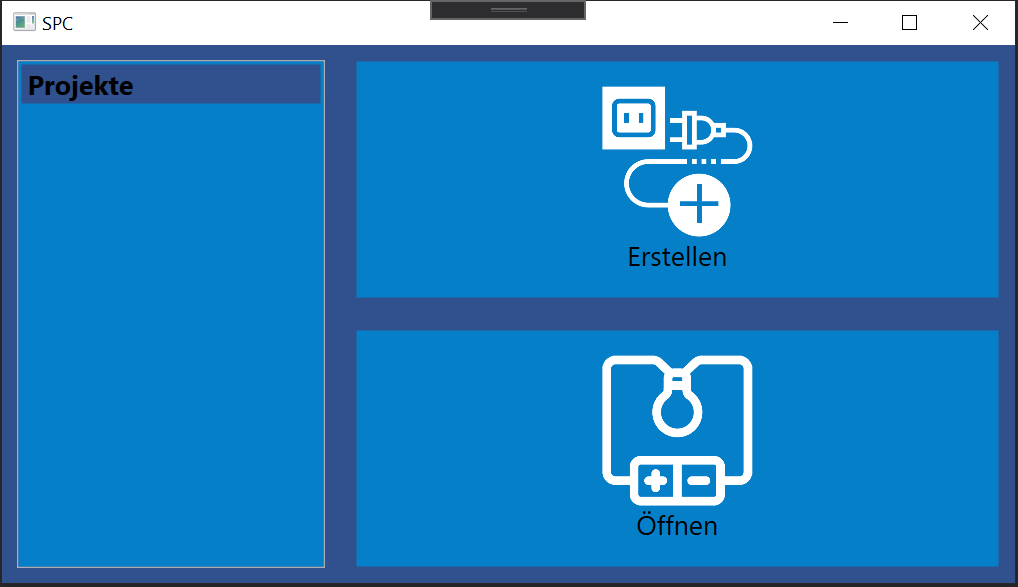
\includegraphics[width=15cm,height=10cm,keepaspectratio]{5Implementierungen/Bilder/StartMenuView.png}
    \caption{Startmenü View}
\end{figure}
\\
Um den Prozess, ein Projekt zu erstellen, fließend übergehen zu lassen wird zwischen der Startmenu-Seite und dem eigentlichen Editor eine zusätzliche
Komponente benötigt, die zwischen den Komponenten transferiert und alle benötigten Informationen von dem Benutzer einholt, benötigte Ressourcen generiert und lädt. 
\pagebreak
\\Beim betätigen des Erstellen-Buttons wird das UserControl der \textit{ProjektNameEingabeView}-Seite aufgerufen. In diesem Schritt der 
Applikation kann der Benutzer dem Projekt einen Namen vergeben und die Datei so im Verzeichnis anlegen. Die dazugehörige GUI beinhaltet eine 
schlichte und einfach gehaltene Eingabemaske, in der lediglich ein Textfeld zur Eingabe des Projektnamens vorhanden ist. Ebenso ist diese mit zwei Buttons versehen die jeweils 
den Prozess zum einen voranbringen durch den (\textit{WeiterButton}) oder zum anderen auf den vorherigen Stand zurückgehen, indem der (\textit{ZurueckButton}) gedrückt wird.
\\
\linebreak
\begin{figure}[htb!]
    \centering
    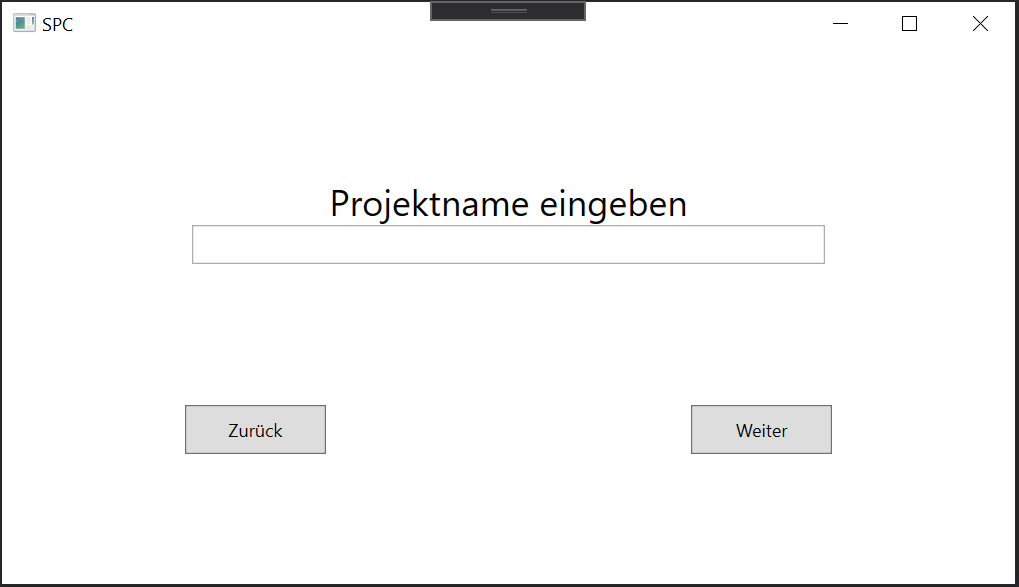
\includegraphics[width=15cm,height=10cm,keepaspectratio]{5Implementierungen/Bilder/ProjektNameEingabeView.png}
    \caption{Projektname View}
\end{figure} 
\pagebreak 
\\Der Code-Ausschnitt zeigt eine vereinfachte From des implementierten UserControls der Eingabe eines Projektnamens. Dabei wurde der \textit{Code behind} weggelassen, da 
in diesem Fall nur das Frontend-Design betrachtet wird. 
\\Dies kann der folgenden Abbildung entnommen werden.
\\
\begin{lstlisting}[language=XML,
    frame=single,           % Ein Rahmen um den Code
    framexleftmargin=15pt,  % Rahmen link von den Zahlen
    style=algoBericht,
    label={startmenuview},
    captionpos=b,           % Caption unter den Code setzen
caption={Projektname-View XAML-Code}]
<UserControl    
    DataContext="{Binding Main, Source={StaticResource Locator}}">
    <Grid>
        <Grid>
            <Grid.RowDefinitions>
                <RowDefinition/>
                <RowDefinition/>
                <RowDefinition/>
            </Grid.RowDefinitions>
            <Grid.ColumnDefinitions>
                <ColumnDefinition/>
                <ColumnDefinition/>
            </Grid.ColumnDefinitions>
            <TextBlock Text="Projektname eingeben" Grid.ColumnSpan="2" 
            FontSize="24" 
            TextAlignment="Center" 
            HorizontalAlignment="Center" VerticalAlignment="Bottom"/>
            <TextBox Grid.Column="0" x:Name="ProjektNameTextFeld"/>
            <Button Grid.Column="0"  x:Name="ZurueckButton" 
            Grid.Row="2" Content="Zurueck"/>
            <Button x:Name="WeiterButton" Grid.Row="2" 
            Grid.Column="1" Content="Weiter"/>
        </Grid>
    </Grid>
</UserControl>
\end{lstlisting}
Als Transferseite wurde diese vom Design unaufmerksam gehalten, da ein Benutzer in der Regel nicht viel Zeit auf dieser Seite aufwenden muss.
Nach dem Ausfüllen des Textblocks und der Bestätigung durch den \textit{WeiterButton} wird der Benutzer direkt auf den eigentlichen Editor weitergeleitet und ist somit in der 
Hauptansicht der eigentlichen Anwendung. 

\subsection{Backend (Simon Leitl)}
Für die Funktionalität des Startmenüs sind mehrere Klassen verantwortlich. Nach MVVM-Prinzip findet die Logik innerhalb der 
ViewModel-Klassen statt. Speziell für das Startmenü lassen sich die Funktionalitäten in drei Bereiche aufteilen.
\begin{itemize}
    \item Das erstellen eines neuen Projekts
    \item Die Anzeige der gespeicherten Projekte im automatisch generierten Projektordner  
    \item Das öffnen eines gespeicherten Projekts
\end{itemize}
Der Nutzer hat die Möglichkeit ein neues 
Projekt über die Schaltfläche \textit{Erstellen} zu erstellen. Hierbei muss im Hintergrund des 
Programms eine neue Datei angelegt werden. Die Datei wird später Daten enthalten, mit welchen die Schaltpläne gespeichert werden können. 
Da der Aufwand ein eigenes Dateiformat zu erstellen für diese Arbeit zu hoch wäre, wird das Textdatei (txt) Format verwendet. Dies eignet 
sich um die Daten der Zeichnung abzuspeichern. Mithilfe von Input/Output Streams ist es so möglich, die Daten in die Textdatei zu schreiben 
und zu lesen. Um die gespeicherten Projekte an einem gemeinsamen Ort abzulegen wird zunächst beim ersten Ausführen, automatisch ein Ordner 
erstellt. In diesem werden zukünftig die neu erstellten Projekte, also Textdateien, abgelegt. 
Um den gesamten Prozess zu starten wird im Startmenu \textit{Erstellen} ausgewählt. Von dort wird man innerhalb des Fensters 
weitergeleitet auf die Benutzeroberfläche ProjektNameEingabeView, welche die Möglichkeit bietet ein Projektname über das vorhandene 
Eingabefeld einzugeben. Über den Button \textit{weiter} wird das Projekt erstellt. Hierbei wird innerhalb der Logik ein RelayCommand 
ausgeführt. Dieser kommuniziert die Interaktion über das, in der XAML festgelegten, Binding. Die Logik wird in der 
ProjektnameEingabeViewModel Klasse als Methoden abgebildet und ausgeführt. Wird also mit dem Button \textit{weiter} interagiert, 
so wird die Methode \textit{NewProjektCommand} im folgenden Code \refname{NewProjektCommand} aufgerufen. 
\linebreak
\begin{lstlisting}[language=C,
    frame=single,           % Ein Rahmen um den Code
    framexleftmargin=15pt,  % Rahmen link von den Zahlen
    style=algoBericht,
    label={NewProjektCommand},
    captionpos=b,           % Caption unter den Code setzen
    caption={NewProjektCommand}]
    public RelayCommand NewProjektCommand { get; private set; }
\end{lstlisting}
Über die enthalten get Methode wird die Interaktion übergeben. Der RelayCommand selbst ruft eine weitere Methode zur Ausführung auf.
\\
\begin{lstlisting}[language=C,
    frame=single,           % Ein Rahmen um den Code
    framexleftmargin=15pt,  % Rahmen link von den Zahlen
    style=algoBericht,
    label={CreateNewProject},
    captionpos=b,           % Caption unter den Code setzen
    caption={CreateNewProject}]
    public void CreateNewProject()
        {
            if (CheckProjectDirectory() == true)
            {
                CreateProjectFile();
            }
            else
            {
                CreateProjectDirectory();
                CreateProjectFile();
            }
        }

\end{lstlisting}
Die Methode \textit{CreateNewProject} ist der Startpunkt der Ablauffolge um eine neues Projekt und damit eine neue Datei zu erstellen. 
Es überprüft zunächst ob der Ordner, in dem die Dateien erzeugt werden sollen, vorhanden ist. Dies gelingt über eine if-Abfrage, die den 
boolschen zurückgegebenen Wert einer Methode auf Richtigkeit überprüft. Bei der Methode handelt es sich um die nachfolgende Methode mit 
dem Namen \textit{CheckProjectDirectory}. Sie gibt \textit{true/false} als Ausgabe zurück. Der Ordner für gespeicherte Dateien, sollte 
sich im selben Pfad bzw. Ablageort befinden wie die ausführende kompilierte .exe des Programms. 
\pagebreak
\begin{lstlisting}[language=C,
    frame=single,           % Ein Rahmen um den Code
    framexleftmargin=15pt,  % Rahmen link von den Zahlen
    style=algoBericht,
    label={CheckProjectDirectory},
    captionpos=b,           % Caption unter den Code setzen
    caption={CheckProjectDirectory}]
    public Boolean CheckProjectDirectory()
    {
       return Directory.Exists("Savings");
    }

\end{lstlisting}
Ist der Rückgabewert \textit{true} wird eine weitere Methode \textit{CreateProjectFile} ausgeführt. Diese enthält Funktionen zum 
erstellen der Datei. Wird \textit{false} zurückgegeben, ist das Verzeichnis nicht vorhanden und muss mittels der Methode 
\textit{CreateProjectDirectory} erstellt werden. 
\\
\begin{lstlisting}[language=C,
    frame=single,           % Ein Rahmen um den Code
    framexleftmargin=15pt,  % Rahmen link von den Zahlen
    style=algoBericht,
    label={CreateProjectDirectory},
    captionpos=b,           % Caption unter den Code setzen
    caption={CreateProjectDirectory}]
    public void CreateProjectDirectory()
        {
            Directory.CreateDirectory("Savings");

        }
\end{lstlisting}
CreateProjectDirectory nutzt System.IO.Directory für 
das Erstellen des Verzeichnisses. Das Verzeichnis soll mit dem Namen 
\textit{Savings} erstellt werden. 
\linebreak
Jetzt wurde sichergestellt, dass das Verzeichnis zum speichern der Dateien existiert und verfügbar ist. Im nächsten Schritt wird die 
Datei erzeugt. Hierfür dient die \textit{CreateProjectFile} Methode. Zunächst wird allerdings der vom Benutzer gewählte Projektname 
benötigt. Dieser kann über die  Benutzereingabe erlangt werden. Hierfür wurde eine weitere Methode implementiert, welche an die View gebindet wurde. 
\\
\begin{lstlisting}[language=C,
    frame=single,           % Ein Rahmen um den Code
    framexleftmargin=15pt,  % Rahmen link von den Zahlen
    style=algoBericht,
    label={ProjektName},
    captionpos=b,           % Caption unter den Code setzen
    caption={ProjektName}]
    public string ProjektName
    {
        get { return projektName; }
        set { projektName = value; }
    }
\end{lstlisting}
Sie gibt den Eingabewert des Nutzer zurück und speichert ihn in einer globalen Variable \textit{projektName}. Diese Variable wird 
im folgenden dazu verwendet die Datei mit dem eingegebenen Namen zu erzeugen.
\\
\begin{lstlisting}[language=C,
    frame=single,           % Ein Rahmen um den Code
    framexleftmargin=15pt,  % Rahmen link von den Zahlen
    style=algoBericht,
    label={ProjektName},
    captionpos=b,           % Caption unter den Code setzen
    caption={ProjektName}]
    public void CreateProjectFile()
    {
        String path = "Savings/" + projektName + ".txt";
        using (FileStream fs = File.Create(path)){}
        MainEditorWindowView mw = new MainEditorWindowView();
        mw.Show();
    }
\end{lstlisting}
Im ersten Schritt der Methode wird der Pfad definiert, der 
benötigt wird um die Datei abzulegen. Hierbei wird der 
Name des Verzeichnis angegeben sowie der Name des Projekts und die Dateiendung. Über einen \textit{Filestream} wird dann die Datei, 
mit dem zuvor festgelegten Pfad erzeugt. Da dies der abschließende Schritt beim Erstellen eines neuen Projektes war, muss das die 
nächster Benutzeroberfläche geladen werden. Es handelt es sich um den Editor. Eine neue Instanz des MainEditorWindowView wird erstellt 
und durch den Befehl \textit{Show()} geöffnet. 
\linebreak
\linebreak
Die zweite Funktion des Startmenü beinhaltet die Anzeige der gespeicherten Projekte. Sie soll einen schnellen Zugriff auf die 
vorhandenen Projekte gewährleisten. Hierzu werden die Projektdateien in Form einer Liste untereinander ausgegeben. Für die 
Implementierung dieser Funktion müssen also alle Dateien, die innerhalb des Verzeichnis liegen, abgerufen und auf der 
Benutzeroberfläche ausgegeben werden. Da es Möglich ist ganze Listen an die View zu binden, werden die Dateinamen in einer Liste 
gespeichert. Die Implementierung befindet sich in der MainViewModel-Klasse des Startmenü. 
\\
\begin{lstlisting}[language=C,
    frame=single,           % Ein Rahmen um den Code
    framexleftmargin=15pt,  % Rahmen link von den Zahlen
    style=algoBericht,
    label={showProjekte},
    captionpos=b,           % Caption unter den Code setzen
    caption={showProjekte}]
        public void showProjekte()
        {
            string path = @"\Savings";
            
            ProcessDirectory(path);
            splitString();
        }
\end{lstlisting}
In der Methode \textit{showProjekte} ist zunächst der Pfad für den Ort des Verzeichnis deklariert. Mit diesem wird eine weitere 
Methode \textit{ProcessDirectory(path)} aufgerufen. Durch diese Methode werden alle Dateien innerhalb des Verzeichnis in eine Liste 
geschrieben. 
\\
\begin{lstlisting}[language=C,
    frame=single,           % Ein Rahmen um den Code
    framexleftmargin=15pt,  % Rahmen link von den Zahlen
    style=algoBericht,
    label={ProcessDirectory},
    captionpos=b,           % Caption unter den Code setzen
    caption={ProcessDirectory}]
    public void ProcessDirectory(string targetDirectory)
    {
        // Process the list of files found in the directory.
        string[] fileEntries = Directory.GetFiles(targetDirectory);

        foreach (string fileName in fileEntries)  
        filePaths.Add(fileName);                  
    }
\end{lstlisting}
Über die in System.IO enthalten Methode \textit{Directory.GetFiles(Path)} werden alle Dateien die innerhalb des zuvor definierten Pfad liegen, ausgegeben. Hier werden diese gleich in einen Array \textit{fileEntries} gespeichert. Mithilfe einer Schleife werden die einzelnen Dateinamen in eine weitere Liste \textit{filePaths} geschrieben, welche global definiert wurde. Da die Methode den vollständigen Dateipfad und nicht nur den Namen der Datei ausgibt, muss der \textit{String} zerteilt werden. Dafür wird der String im nachfolgenden Code gesplittet. 
\pagebreak
\begin{lstlisting}[language=C,
    frame=single,           % Ein Rahmen um den Code
    framexleftmargin=15pt,  % Rahmen link von den Zahlen
    style=algoBericht,
    label={splitString},
    captionpos=b,           % Caption unter den Code setzen
    caption={splitString}]
    public void splitString()
        {
            for (int i = 0; i < filePaths.Count; i++){
                string name = filePaths[i];
                string[] split = Regex.Split(name, "\\");
                _files.Add(split[split.Length-1]);
                }
        }
\end{lstlisting}
Die Liste \textit{filePaths}, welche Global definiert wurde und die Dateipfade beinhaltet wird hier über \textit{Regex.Split()} aufgeteilt. Die Bedingung für die Aufteilung ist der sogenannte Backslash \textbackslash. Jedesmal wenn innerhalb der Zeichenkette ein Backslash erscheint, wird an dieser Stelle geteilt und als neue Position in die Liste geschrieben. Da der Dateiname der letzte Teil des Pfads ist, kann der letzte Eintrag der Liste als Dateinamen ausgewählt werden. Damit alle Einträge der Liste gesplittet und in die neue Liste \textit{files} eingetragen werden, wird in einer Schleife über die Liste iteriert. \textit{files} wird in der folgenden Methode dazu genutzt um an die View anhand eines Bindings übergeben zu werden. 
\\
\begin{lstlisting}[language=C,
    frame=single,           % Ein Rahmen um den Code
    framexleftmargin=15pt,  % Rahmen link von den Zahlen
    style=algoBericht,
    label={getFileList},
    captionpos=b,           % Caption unter den Code setzen
    caption={getFileList}]
    public ObservableCollection<string> getFileList
    {
        get
        {
            return _files;
        }
    }
\end{lstlisting}
Die Methode \textit{getFileList} liefert die Liste mit den Dateinamen als Observablecollection zurück. Das UI Element kann über ein Binding zu dieser Methode die Namen auf der Benutzeroberfläche abbilden.  
Ein Code-Ausschnitt der Listenansicht-Implementierung soll einen Einblick verschaffen wie die \textit{Starmenu-XAML} in Bezug auf die Liste aufgebaut und 
Über die in System.IO enthalten Methode \textit{Directory.GetFiles(Path)} 
werden alle Dateien die innerhalb des zuvor definierten Pfad 
liegen, ausgegeben. Hier werden diese gleich in einen Array \textit{fileEntries} gespeichert. Mithilfe einer Schleife werden die einzelnen 
Dateinamen in eine weitere Liste \textit{filePaths} geschrieben, welche global definiert wurde.
\\
Ein Code-Ausschnitt der Listenansicht-Implementierung soll einen Einblick verschaffen wie die 
\textit{Starmenu-XAML} in Bezug auf die Liste aufgebaut und 
implementiert ist.
\\
\pagebreak
\section{Use Case 2: Toolbox}
Nachdem die Dateien und Objekte zur Erstellung eines Projekts implementiert waren, wurde sich dem Frontend des Editors gewidmet, um die eigentlichen
Funktionen bereitzustellen, damit die Implementierung des Editors umgesetzt werden konnte. 
\\Parallel zu dem Design des Startmenüs wurden ebenso die grafische Darstellung 
des Editors erstellt. Das dazugehörige MockUp wurde in Kapitel 4 Abbildung 4.4 bereits erwähnt und genauestens beschrieben. 
Da die Überlegungen zum Design im Voraus getätigt und eine visuelle Vorarbeit geleistet wurde, konnte sich bei der Entwicklung lediglich an dem 
grafisch dargestellten Entwurf orientiert werden.
\subsection{Frontend (Mikka Jenne)}
Das UI-Element des Editors besteht grundlegend aus einem \textit{Window-XAML} und ist in ein Raster aufgeteilt. Um das Raster zu verdeutlichen, wird die Definition dieses Rasters aufgeführt.
\\ 
\begin{lstlisting}[language=XML,
    frame=single,           % Ein Rahmen um den Code
    framexleftmargin=15pt,  % Rahmen link von den Zahlen
    style=algoBericht,
    label={usercontrolsnippet},
    captionpos=b,           % Caption unter den Code setzen
caption={Editor Raster-Layout}]
<Grid.ColumnDefinitions>
    <ColumnDefinition/>
    <ColumnDefinition/>
    <ColumnDefinition/>
    <ColumnDefinition/>
    <ColumnDefinition/>
    <ColumnDefinition/>
    <ColumnDefinition/>
    <ColumnDefinition/>
</Grid.ColumnDefinitions>
<Grid.RowDefinitions>
    <RowDefinition Height="0.3*"/>
    <RowDefinition/>
    <RowDefinition/>
    <RowDefinition/>
    <RowDefinition/>
    <RowDefinition/>
    <RowDefinition/>
    <RowDefinition/>
</Grid.RowDefinitions>
\end{lstlisting}
Mit dieser Implementierung wird das \textit{Window} in ein Raster aufgeteilt mit Rechtecken gleicher Größe. Durch Verschmelzung einzelner Rechtecke können 
größere Flächen gebildet werden, um dementsprechend mehr Inhalt darin anzeigen zu können. So kann z.B. ein \textit{UserControl} referenziert werden,
welches viel Platz benötigt. In dem Fall des Editors ist das die eigentliche Zeichenfläche.
\\ 
\\Das Editor-Element ist als ein separates 
\textit{Window} angelegt. Es öffnet sich nach dem betätigen des \textit{WeiterButton} des \textit{UserControls-ProjektNameEingabe} ein neues Fenster mit der Editor Ansicht. 
Auf diesen Schritt wird nicht weiter drauf eingegangen, da diese Aktion über das Backend verwaltet wird. 
\pagebreak
\\Der aktuelle Entwurf des Editors ist in folgender Abbildung zu entnehmen. Die Umsetzung ähnelt der Abbildung 4.4 in grundlegenden Struktur.
\begin{figure}[hbt!]
    \centering
    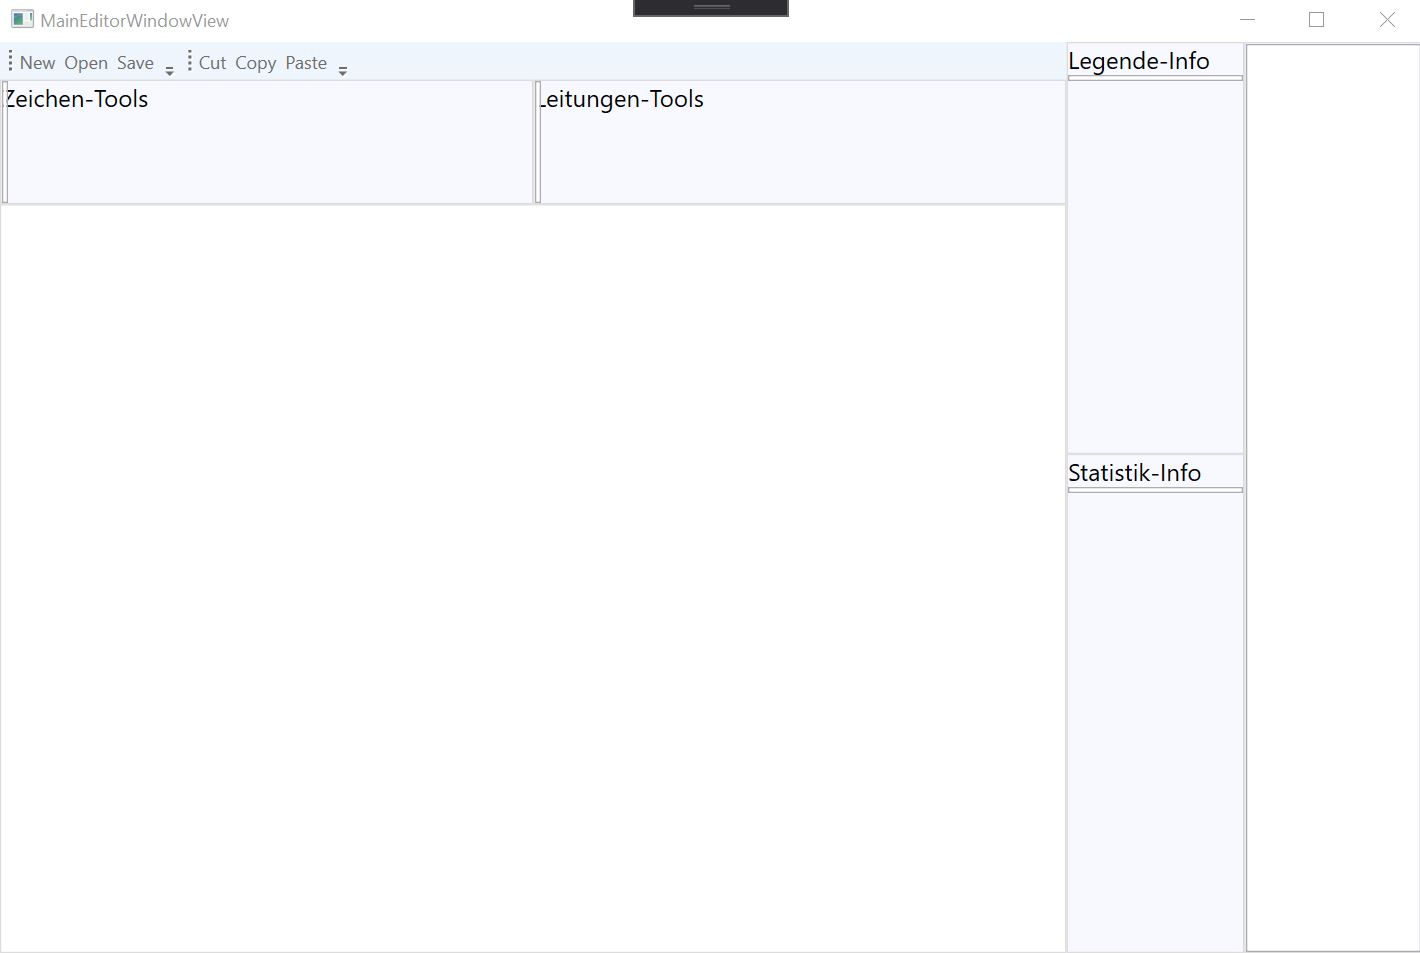
\includegraphics[width=15cm,height=10cm,keepaspectratio]{5Implementierungen/Bilder/EditorView.JPG}
    \caption{Editor View}
\end{figure}
\\Die \textit{Window}-Datei ist durch eine Anreihung von \textit{Grid-Elementen} strukturiert und in sieben unterschiedlich große Flächen gegliedert. Die 
Rasterelemente sind für eine jeweilige Komponente als Platzhalter gedacht, bzw. für ein bestimmtes \textit{UserControl} vorgemerkt. Alle Komponenten 
sind als ein \textit{UserControl} ausgelagert, um die Code-Struktur der Hauptseite zu entlasten und übersichtlicher zu gestalten.
\\Das \textit{Window-XAML}-Element is so als zentraler Ort für alle \textit{UserControls} bestimmt.
\\
\pagebreak
\\In folgender Abbildung wird die Aufteilung der einzelnen Felder in der \textit{XAML}-Datei veranschaulicht.
Um genauer zu verdeutlichen wie die einzelnen \textit{UserControls} in dem Editor-Fenster integriert werden, wird ergänzend zu der Abbildung 5.3 ein Code-
Ausschnitt von einer der \textit{UserControls} aufgeführt.
\\
\begin{lstlisting}[language=XML,
    frame=single,           % Ein Rahmen um den Code
    framexleftmargin=15pt,  % Rahmen link von den Zahlen
    style=algoBericht,
    label={usercontrolsnippet},
    captionpos=b,           % Caption unter den Code setzen
caption={UserControl-Referenz Code-Auschnitt}]
<Window
    xmlns:local="clr-namespace:SPC3.SPC.Editor.Views">
    <DockPanel Grid.Column="0" Grid.Row="2" 
     Grid.RowSpan="6" Grid.ColumnSpan="6">
        <Grid>
            <local:ZeichenFlacheView x:Name="ZeichenFlaecheView"/>
        </Grid>
    </DockPanel>
</Window>
\end{lstlisting}
Der Verweis durch \textit{local} gibt Informationen darüber in welchem Namespace oder genauer in welchem Ordner des Projekts dieses Objekt zu finden ist, um das Element 
referenzieren zu können. Durch diesen Aufruf wird dem Hauptfenster eindeutig mitgeteilt welche Klasse, konkret welches \textit{UserControl} in diesem Feld 
geladen werden soll.
Auf diese Weise werden alle \textit{UserControls} in die \textit{MainWindow-XAML}-Datei geladen.

\begin{lstlisting}[language=XML,
    frame=single,           % Ein Rahmen um den Code
    framexleftmargin=15pt,  % Rahmen link von den Zahlen
    style=algoBericht,
    label={startmenuview},
    captionpos=b,           % Caption unter den Code setzen
caption={Startmenu-Recent-Projects-Code}]
<ListView Grid.Column="0" x:Name="viewUsedProjects" Background="#067FC9" 
    Margin="10">
    <ListView.ItemTemplate>
        <DataTemplate>
            <WrapPanel>
                <TextBlock Text="{Binding ProjektPfad}"></TextBlock>
            </WrapPanel>
        </DataTemplate>
    </ListView.ItemTemplate>
    <ListViewItem Background="#31508E" FontWeight="Bold" FontSize="18">
    Projekte</ListViewItem>
</ListView>
\end{lstlisting}
Das ListView-Item wird eindeutig einer \textit{Grid.Column} zugeordnet und mit einer \textit{Background-Color} Farbe versehen. 
Zusätzlich wird dem Element
einen Namen vergeben, um bei einer Referenzierung das Objekt eindeutig ansprechen zu können.
\\Der Ausschnitt zeigt, wie der Aufruf, bzw. das \textit{Binding} eines Objekts, in dem Fall das dynamisch generierte \textit{ListView-Item}, 
angebunden und auf den Code im Backend verwiesen wird. 
\pagebreak
\subsection{Backend (Simon Leitl)}
Die Toolbox-Werkzeug beeinhalten, wie bereits innerhalb dieser Arbeit erwähnt, Funktionen und Komponten die nötig sind um den Schaltplan zu zeichnen. Der Aufbau der Elemente innerhalb der Toolboxen wird im folgenden Abschnitt exemplarisch anhand der Elektronischen Komponenten erläutert. 
\begin{figure}[hb]
    \centering
    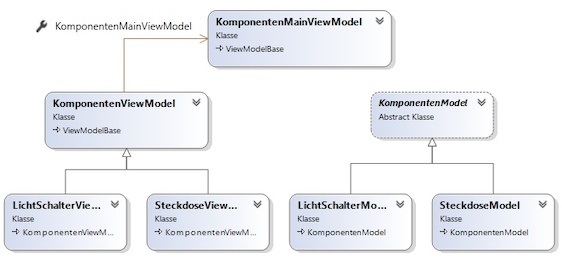
\includegraphics[width=500px,height=193px]{5Implementierungen/Bilder/ClassDiagram1}
    \caption{Klassendiagramm Toolbox}
    \label{pic:klassendiagramm-toolbox}
\end{figure}
\linebreak
Das oberhalb abgebildetet Klassendiagramm gibt die Klassen, welche die Komponenten repräsentieren wieder. Auch hier lassen sich wieder Models und ViewModels gemäß MVVM wiederfinden. Dabei enthalten die Models die Struktur einer Komponente. In diesem Fall den Namen der Komponenten, sowie Eigenschaften des Symbols. Die ViewModels dienen dazu die Struktur der KomponentenModels abzubilden und mit einer Logik zu versehen. Außerdem werden die einzelnen Komponenten später über die ViewModels aufgerufen, da nicht direkt mit den Models kommuniziert wird. Denn diese sollen nur die Datenstruktur festlegen.
In diesem Beispiel werden zwei Komponenten behandelt. Ein Lichtschalter und eine Steckdose sollen zur Verfügung gestellt werden. Diese sollen später in den Schaltplan integriebar sein. Beide Klassen, LichtSchalterModel und SteckdoseModel erben von der abstrakten Klasse KomponentenModel. Die abstrakte Klasse gibt die allgemeine Struktur für die Models der Komponenten vor. Wenn eine weitere Komponente hinzugefügt werden soll, muss jediglich ein Model erstellt werden, das von der abstrakten KomponentenModel Klasse erbt. Die Methoden und Eigenschaften sind dann aufgrund der Vererbung vorgegeben. Somit gelingt eine einfache Erweiterung.
\pagebreak
\begin{lstlisting}[language=C,
    frame=single,           % Ein Rahmen um den Code
    framexleftmargin=15pt,  % Rahmen link von den Zahlen
    style=algoBericht,
    label={KomponentenModel},
    captionpos=b,           % Caption unter den Code setzen
    caption={KomponentenModel}]
    abstract class KomponentenModel
    {
        public KomponentenModel(){}

        public String komponentenName;
        private String komponentenBeschreibung;
        private String symbolPfad;

        public String KomponentenName
        {
            get -> komponentenName;
            set -> komponentenBeschreibung = value;
        }


        public String KomponentenBeschreibung
        {
            get -> komponentenBeschreibung;
            set -> komponentenBeschreibung = value;
        }

        public String symbolPfad
        {
            get -> symbolpfad;
            set -> symbolPfad = value;
        }
    }
\end{lstlisting}
Der konkrete Aufbau für eine KomponentenModel Klasse kann dem Code-Beispiel 5.15 entnommen werden. Es werden zunächst die Eigenschaften als drei globale Felder in Form von \textit{String} deklariert. Sie enthalten den Namen, eine Beschreibung und den Pfad zur Bilddatei der Komponente. Über öffentliche Getter- und Settermethoden ist es Möglich die Eigenschaften zu setzen und zu lesen. Es wird allerdings nicht empfohlen die Eigenschaften innerhalb des Systems zu ändern. Eine Änderung wird nur innerhalb der Modelklasse empfohlen. Die Methode wird jedoch implementiert um sie in möglichen Fällen bereitzustellen. 
\pagebreak
\begin{lstlisting}[language=C,
    frame=single,           % Ein Rahmen um den Code
    framexleftmargin=15pt,  % Rahmen link von den Zahlen
    style=algoBericht,
    label={KomponentenModel},
    captionpos=b,           % Caption unter den Code setzen
    caption={KomponentenModel}]
    class LichtSchalterModel : KomponentenModel
    {
      private string komponentenName = "Lichtschalter";
      private string symbolPfad = @"\KomponentenPictures\lichtschalter.png";

      public string getKomponentenName()
      {
          return komponentenName;
      }

      public string getSymbolPfad()
      {
          return symbolPfad;
      }
    }
\end{lstlisting}
Im Code-Beispiel 5.16 ist die konkrete Ausführung einer KomponentenModel Klasse dargestellt. Hier wird der Name, sowie der Symbolpfad festgelegt. Mithilfe von Gettermethoden werden diese zurückgegeben und bereitgestellt, sodass sie von den ViewModels im benutzt und implementiert werden können.
\begin{lstlisting}[language=C,
    frame=single,           % Ein Rahmen um den Code
    framexleftmargin=15pt,  % Rahmen link von den Zahlen
    style=algoBericht,
    label={LichtSchalterViewModel},
    captionpos=b,           % Caption unter den Code setzen
    caption={LichtSchalterViewModel}]
    public class LichtSchalterViewModel : KomponentenViewModel
    {
        LichtSchalterModel lichtSchalterModel = new LichtSchalterModel();
        public LichtSchalterViewModel()
        {
            Name = lichtSchalterModel.getKomponentenName();
            Symbol = lichtSchalterModel.getSymbolPfad();
        }
    }
\end{lstlisting}
Parallel zur Model Klasse einer Komponente, in diesem Fall der Steckdose, gibt es eine ViewModelKlasse der Komponente. Diese trägt den Klassennamen LichtSchalterViewModel. Sie implementiert, die im nachfolgenden Code-Beispiel 5.18 beschriebene KomponentenViewModel Klasse. Um die Daten der Model Klasse zu nutzen bildet die LichtSchalterViewModel Klasse eine Instanz ihrer zugehörigen Model Klasse. Mit dieser Instanz werden die Daten anhand der definierten Gettermethoden abgerufen. 
\pagebreak
\begin{lstlisting}[language=C,
    frame=single,           % Ein Rahmen um den Code
    framexleftmargin=15pt,  % Rahmen link von den Zahlen
    style=algoBericht,
    label={KomponentenViewModel},
    captionpos=b,           % Caption unter den Code setzen
    caption={KomponentenViewModel}]
    public class KomponentenViewModel : ViewModelBase
    {
        public string _name;
        public string _symbol;


        public string Name
        {
            get { return _name;}
            set { Set(() -> Name, ref _name, value); }
        }

       public string Symbol
        {
            get { return _symbol; }
            set { Set(() -> Symbol, ref _symbol, value); }
        }

        public KomponentenMainViewModel KomponentenMainViewModel
        {
            get -> default(KomponentenMainViewModel);
            set{}
        }
\end{lstlisting}
Betrachtet man nun die KomponentenViewModel Klasse, welche in Code-Beispiel 5.18 dargestellt wird, lässt sich eine Ähnlichkeit zu den Models erkennen. Diese ViewModel Klasse stellt die Methoden zur Verfügung um den Namen sowie den Pfad des Symbols, einer Komponenten, aus dessen ViewModelKlasse zu lesen. Diese Methode hätten prinzipiell auch im ViewModel der Komponenten definiert werden können. Sprich das LichtSchalterViewModel hätte selbst diese Getter- und Settermethoden implementieren können. Allerdings wäre das dann bei jedem weiteren ViewModel einer Komponente nötig. Um duplizierten Code einzusparen wurden diese Methoden ausgelagert in die KomponentenViewModel Klasse im Code-Beispiel 5.18. Sie kann einfach in allen weiteren ViewModelKlassen der Komponenten implementiert werden und so die Namen und Symbolpfade abrufen.  
\linebreak
\linebreak
Jetzt wo geklärt ist, wie die Daten aus den Models gewonnen werden können, fehlt noch die eigentliche Logik. Im nächsten Schritt sollen die Komponenten mit ihren Namen und Symbolen in einer Liste auf der Benutzeroberfläche bereitgestellt werden. Dazu sollen die einzelnen ViewModels in eine Liste geladen werden. Hierfür ist die KomponentenMainViewModel Klasse vorhanden. Sie vereint die gemeinsame Logik, so wie den gemeinsamen Gebrauch der einzelnen ViewModelKlassen in einem. Außerdem werden ihre Methoden an die Benutzeroberfläche gebindet. Um in MVVM ViewModels global im Projekt bereitzustellen gibt es eine ViewModelLocator Klasse. Sie wird verwendet um die ViewModels zu lokalisieren und innerhalb des gesamten Projekts bereitzustellen. Dies hat zum Vorteil, dass die ViewModel Klassen nicht jedesmal bei Gebrauch einzeln instanziert werden müssen. Neben der Backend Implementierung nutzen auch die XAML Dateien des Frontends den ViewModelLocator um die Quelle ihrer Bindings festzulegen.
\begin{lstlisting}[language=C,
    frame=single,           % Ein Rahmen um den Code
    framexleftmargin=15pt,  % Rahmen link von den Zahlen
    style=algoBericht,
    label={viewModelLocator},
    captionpos=b,           % Caption unter den Code setzen
    caption={viewModelLocator}]
    public KomponentenMainViewModel KomponentenMainViewModel
    {
     get
     {
      return ServiceLocator.Current.GetInstance<KomponentenMainViewModel>();
     }
    }
\end{lstlisting}
Eine Instanzierung der KomponentenViewModel Klasse wird in Code-Beispiel 5.19 abgebildet. Es wird eine Instanz der Klasse zurückgegeben, welche dann global im Projekt verwendet werden kann. Im nächsten Code-Beispiel 5.20 kommt diese Instanz zum Einsatz. Hier wird eine ObservableCollection verwendet, die alle Instanzen der KomponentenViewModel Klasse bündelt und in einer Liste ausgibt. 
\begin{lstlisting}[language=C,
    frame=single,           % Ein Rahmen um den Code
    framexleftmargin=15pt,  % Rahmen link von den Zahlen
    style=algoBericht,
    label={viewModelList},
    captionpos=b,           % Caption unter den Code setzen
    caption={viewModelList}]
    public ObservableCollection<KomponentenViewModel> ViewModelList
    {
        get
        {
            return _viewModelList;
        }
    }
\end{lstlisting}
Die zurückgegebene ViewModelList enthält nun die definierten ViewModels. Über diese ist es möglich die Daten der einzelnen Komponenten zu lesen. Um nun die Namen letztendlich auf der Benutzeroberfläche anzuzeigen, wird eine weitere Methode erstellt welche von der XAML gebindet werden kann. Sie enthält eine Liste vom Typ \textit{String} mit den Namen aller definierten Komponenten. Sie wird im Code-Beispiel 5.21 dargestellt.
\begin{lstlisting}[language=C,
    frame=single,           % Ein Rahmen um den Code
    framexleftmargin=15pt,  % Rahmen link von den Zahlen
    style=algoBericht,
    label={viewModelNameList},
    captionpos=b,           % Caption unter den Code setzen
    caption={viewModelNameList}]
    public List<string> ViewModelNameList
             {
                 get { return _viewModelNameList; }
             } 
\end{lstlisting}
Die ViewModelNameList Methode vom Typ \textit{List<String>} gibt die Liste mit allen Namen der Komponenten zurück. 
\\
Damit die Benutzeroberfläche die Komponenten in einer Liste wiederverwendet und darstellt, wurde die von WPF bereitgestellte ListBox Methode verwendet. Sie gibt die Daten, die sie vom Binding erhält in einer Liste aus.
\begin{lstlisting}[language=XML,
    frame=single,           % Ein Rahmen um den Code
    framexleftmargin=15pt,  % Rahmen link von den Zahlen
    style=algoBericht,
    label={komponentenToolsView},
    captionpos=b,           % Caption unter den Code setzen
caption={KomponentenToolsView XAML-Code}]
<ListBox ItemsSource="{Binding ViewModelList}" 
ItemTemplate="{StaticResource komponenten}"/>
\end{lstlisting}
Als ItemsSource enthält die Listbox die ViewModelList. Dadurch erkennt sie wie viele Komponenten vorhanden sind und wie die Daten eines zugehörigen strukturiert sind. Um nun festzulegen wie die Komponenten innerhalb der Liste angezeigt werden sollen, muss ein Custom Template definiert werden. Diese soll beschreiben, dass zuerst das Symbol und darunter der Name dargestellt werden soll.  
\begin{lstlisting}[language=XML,
    frame=single,           % Ein Rahmen um den Code
    framexleftmargin=15pt,  % Rahmen link von den Zahlen
    style=algoBericht,
    label={komponentenToolsView},
    captionpos=b,           % Caption unter den Code setzen
caption={KomponentenToolsView XAML-Code}]
<DataTemplate x:Key="komponenten">
    <StackPanel>
        <Image Source="{Binding ViewModelSymbolList}"/>
		<TextBlock Text="{Binding ViewModelNameList}"/>
	</StackPanel>
</DataTemplate>
\end{lstlisting}
Hierfür wird ein DataTemplate in den globalen Ressourcen der XAML Datei gebildet. Das Bild wird ales Image ausgegeben und erhält seinen Pfad über das Binden der ViewModelSymbolList Methode. Der Name wird in einem Textblock dargestellt und wird über die ViewModelNameList Methode abgerufen.
\\
\linebreak
In diesem gesamten Verfahren können nun weitere Komponenten hinzugefügt werden. Dafür muss eine Model Klasse mit der Beschreibung der Komponente, sowie eine zugehörige ViewModel Klasse angelegt werden. Die restlichen Strukturen sind vorhanden. So ermöglicht es eine modulare und einfache Erweiterbarkeit für die gesamte Softwarearchitektur. Bei der Toolbox LeitungenTools wurde nach dem selben Prinzip vorgegangen. 
\pagebreak
\section{Use Case 3: Zeichenfläche (Mikka Jenne)}
\subsection{Frontend}
Mit der Fertigstellung der graphischen Benutzeroberfläche des Editors konnte sich an die Arbeit der noch ausstehenden Use Cases gemacht 
werden. Darunter fällt z.B. der obig aufgeführt UC 2, dieser beinhaltet alle relevanten Komponenten die zum Zeichnen 
benötigt werden, bspw. Symbol und Funktion von Lichtschaltern oder Steckdosen o.ä. und der Use Case 3, welcher in diesem Kapitel aufgeführt ist.
\\Explizit handelt es sich bei diesem Anwendungsfall um das individuelle Zeichnen in einem vorgegebenen Bereich. In diesem Fall ist dieser begrenzte 
Bereich ein \textit{Canvas}. Dieser ist in Abbildung 5.4, der Editor-Ansicht, im linken unteren Eck zu entnehmen. Eine große markante Fläche, die 
am meisten Platz beansprucht. Ein Canvas, dt. Leinwand, repräsentiert in \acs{WPF} eine Fläche die explizit als eine Leinwand zum Zeichnen vorgegeben ist und viele Funktionen dazu bereitstellt.
Der Code-Ausschnitt 5.13 zeigt das Canvas, welches als fester Parameter in der \acs{XAML} vorhanden ist. Alle weiteren Änderungen auf dem Canvas werden dynamisch 
erstellt und nachgeladen. Die Funktionsweise und was es mit dem \textit{Interaction.Triggers} auf sich hat wird im Backend genauestens erläutert.
\\
\begin{lstlisting}[language=XML,
    frame=single,           % Ein Rahmen um den Code
    framexleftmargin=15pt,  % Rahmen link von den Zahlen
    style=algoBericht,
    label={usercontrolsnippet},
    captionpos=b,           % Caption unter den Code setzen
caption={UserControl-Referenz Code-Ausschnitt}]
<UserControl>
    <Grid>
        <Grid.RowDefinitions>
            <RowDefinition></RowDefinition>
        </Grid.RowDefinitions>
        <Border Background="GhostWhite" 
         BorderBrush="Gainsboro" BorderThickness="1">
            <Canvas Grid.Row="1" Background="White">
                <i:Interaction.Triggers>
                    <i:EventTrigger EventName="MouseLeftButtonUp">
                        <command:EventToCommand Command="{Binding 
                         GetKooradinatesClickOnCanvas}" 
                         PassEventArgsToCommand="True"/>
                    </i:EventTrigger>
                </i:Interaction.Triggers>   
            </Canvas>
        </Border>
    </Grid>
</UserControl>
\end{lstlisting}
\subsection{Backend}
Der \textit{Interaction.Triggers} ist die Schnittstelle zu der Funktion im Backend, die die Methode zum Zeichnen beinhaltet und aufruft. Mit dem 
\textit{EventToCommand} wird eine Funktion gebindet die in der \textit{ViewModel-Class} implementiert ist. Diese Methode ist als \textit{ICommand}-Methode 
initialisiert und implementiert zu Anfang das Event mit dem der \textit{MouseClick} aufgefangen wird. Dieses MouseClick-Event wird dann auf einen Command gecastet und so an 
das Backend übergeben. 
\\
\begin{lstlisting}[language=C,
    frame=single,           % Ein Rahmen um den Code
    framexleftmargin=15pt,  % Rahmen link von den Zahlen
    style=algoBericht,
    label={icommandclicksnippet},
    captionpos=b,           % Caption unter den Code setzen
caption={ICommand-OnClick Code-Ausschnitt}]
public ICommand GetKooradinatesClickOnCanvas
{
    get { return new RelayCommand<EventArgs>(MouseClick_ToDraw); }
}
\end{lstlisting}
Bei einem MouseClick wird wie oben erwähnt die Funktion \textit{GetKoordinatesClickOnCanvas} aufgerufen, die einen Command returnt, welcher ebenso eine 
Methode beinhaltet in der final der Befehl zum Zeichnen ausgeführt werden soll. 
\\
\begin{lstlisting}[language=C,
    frame=single,           % Ein Rahmen um den Code
    framexleftmargin=15pt,  % Rahmen link von den Zahlen
    style=algoBericht,
    label={mouseclicksnippet},
    captionpos=b,           % Caption unter den Code setzen
caption={MouseClick-Funktion Code-Ausschnitt}]
private void MouseClick_ToDraw(EventArgs args)
{
    MouseEventArgs e = (MouseEventArgs) args;

    if(e.LeftButton == MouseButtonState.Released) // 
    {
        if (TestArrayPosition(mousePosition) == true)
        {
            var position = new Point();
            position = e.GetPosition(e.Device.Target);
            mousePosition[0] = position;
        }
    }
}
\end{lstlisting}
In diesem Ausschnitt wird das Event zu einem \textit{MouseEventArgs} gecastet, um bei dem MouseClick die Koordinaten in dem Canvas bestimmen zu können. 
Dabei wird die jeweilige Position gespeichert. Nach erfolgreicher Überprüfung und Speicherung des zweiten Punkts werden die gespeicherten Koordinaten einer Methode 
des Namespaces System.Drawing übergeben. Die Funktion des System.Drawings nimmt die Koordinaten und wandelt diese zu Punkten um, um sie anschließend 
der \textit{DrawLine()-Methode} zu übergeben. Diese Methode ist ebenso Bestandteil des Namespaces \textit{System.Drawing}. Dieser Ausdruck bekommt alle relevanten Parameter 
übergeben, um schlussendlich eine Linie zeichnen zu können.
\\
\linebreak
Nach dem die Applikation gestartet wurde und das Editor-Fenster erscheint, kann der Benutzer prinzipiell anfangen Linien in das Canvas zu zeichnen. Mit 
diesen Linien werden Grundriss oder Leitungen definiert.
\\
\linebreak
Bei der Aktion des ersten MouseClick werden die ersten Koordinaten abgerufen und in ein Array gespeichert. Bei dem zweiten Klick wird überprüft, ob 
in dem Array schon Werte vorhanden sind und ob die Koordinaten des zweiten Klicks eventuell identisch zu den Koordinaten des ersten Klicks. Falls dieser Fall nicht zutrifft, 
werden die im Array gespeicherten Koordinaten dem \textit{Line}-Parameter übergeben, damit ein \textit{Line}-Objekt erstellt werden kann. 
\linebreak 
Dieser Parameter wird generiert und beinhaltet auch alle zutreffenden Werte, nur kann die Linie aktuell nicht auf der Benutzeroberfläche angezeigt werden.
Prinzipiell sollte der ICommand-Befehl die grafische Benutzeroberfläche bei einem \textit{OnPropertyChanged}-Aufruf den jeweiligen Wert ändern. 
Aus derzeit unerklärlichen Gründen wird die generierte Linie nicht auf das Canvas in der Benutzeroberfläche übertragen. Der Compiler kompiliert alles nach Plan 
und zeigt keine Exception an, bzw. terminiert die Applikation nicht durch einen Error.
\\
\linebreak
Aus zeitlichen Gründen war es im Rahmen dieser Arbeit nicht möglich diesen Fehler genauer zu analysieren und die fehlerhafte Darstellung zu berichtigen.
Eine Erklärung für dieses Verhalten der Applikation, bzw. des Compilers ist nicht vorhanden und müsste erst mit einer detaillierten Recherche analysiert und berichtigt werden. 


%\end{align*}


\chapter{Fazit und Ausblick}
\section{Fazit}
Das Ziel dieser Arbeit war die Grundlage und Architekturkonzeption einer Software zur Erstellung von Schaltplänen zu erarbeiten. Dafür wurden in den ersten Schritten die genauen Anforderungen an das System festgelegt. Darauf basierend wurden mit C\#, .NET und WPF die Technologien ausgewählt. Um eine Modularität zu gewährleisten, damit auch künfigt an der Software weiterentwickelt werden kann, musste ein geeignetes Entwurfsmuster gefunden werden, nach dem die Architektur aufgebaut wird. Mit MVVM wurde ein passendes Muster, dass vorallem für WPF und C\# besonders geeignet ist gefunden. Bevor es in die konkrete Umsetzung ging, wurde die Architektur anhand von Use Cases und Klassendiagrammen modeliert. Anhand dieser Überlegungen konnte dann die Architektur implementiert werden. Eine große Rolle für die Implementierung auf Basis des MVVM Musters hat dabei das MVVM Light Framework gespielt. 
\\
\linebreak
Aufgrund der hohen Entkopplung zwischen den einzelnen Modulen und speziell der Benutzeroberfläche und Logik, wird eine einfachere Wartbarkeit sowie Erweiterbarkeit des Projekts gewährleistet. Aber auch die Möglichkeit die einzelnen Bestandteile zu testen, ist durch die hohe Entkopplung möglich. Neben den Vorteilen bringt die Moldularität auch Nachteile bei der Entwicklung. So traten immer wieder Schwierigkeiten und komplexe Probleme auf, insbesondere in der Verbindung zwischen der Benutzeroberfläche und der Logik. In einzelnen Fällen mussten Synchronisierungen zwischen Benutzeroberfläche und Logik durch Hilfsklassen unterstützt werden. Auch für die Anzeige bestimmter Elemente mussten Converter Klassen geschrieben werden. Änderungen in der Projektstruktur haben teilweise zu komplexen Verschiebungen, vorallem in den Namensräumen innherlab der Visual Studio IDE geführt. Daher wird nicht empfohlen die Struktur in der künftigen Entwicklung groß zu ändern. In dieser Arbeit wurde eine fundierte Grundlage geschaffen, auf der eine Weiterentwicklung stattfinden kann. 
\\
\linebreak
Im gesamten betrachtet bietet das Ergebnis dieser Arbeit einen klaren und leicht verständlichen Systemaufbau und die Grundlage für Weiterentwicklungen. Hält man sich an das vorgegebene Muster sowie die bisherig implementierte Struktur des Projekts, gelingt das Hinzufügen weiterer Funktionen einfach und erfolgreich.
\\
\section{Ausblick}
Bisher bietet die Software die Möglichkeit neue Projekte anzulegen. Dabei erzeugt das System automatisch eine Projektdatei. Nachdem ein Projekt angelegt wurde, öffnet sich der Editor. Er stellt die Eigentliche Funktionalität des Programms dar. Der Editor hat die grafische Struktur für alle nötigen Funktionen implementiert. Eine Struktur der Komponenten für die Toolbox der Elektro-Komponenten liegt ebenfalls vor und kann beliebig erweitert werden. Auch die Zeichenfläche ist verfügbar. Sie erkennt die Mausposition und registriert einen Klick. Dabei wird die Position gespeichert und anhand der zwei Positionen, eine Linie gezeichnet. Die Linie existiert im Programmcode, wird allerdings bislang noch nicht an der Benutzeroberfläche angezeigt.
\\ 
In weiteren Entwicklungen können die Funktionalitäten erweitert werden. Auf Basis des Systems kann ein Speicherverfahren implementiert werden, dass die Zeichnungen innerhalb der vorhandenen Text-Datei abspeichert. Die Möglichkeit Schaltpläne zu zeichnen kann ebenfalls Funktional erweitert werden. So ist das langfristige Ziel vollständige 2D Schaltpläne zu entwerfen, die in einem fertigen Format (z.B. PDF) exportiert werden können. Eine weitere Konzeption sieht vor, die Schaltpläne in einer 3D Sicht abzubilden um festzustellen, wo genau innerhalb eines Gebäudes bestimmte Komponenten angebracht werden können. Abschließend lässt sich sagen, dass die Grundlage und vorallem eine grundlegene Architektur innerhalb dieser Arbeit erstellt und entwickelt wurden. Diese können als ausreichende Basis für zukünftige Entwicklungen genutzt werden um ein vollständiges, für den Anwender bestimmtes Programm zu erstellen.



% Ab hier beginnt der Anhang
\appendix
\addcontentsline{toc}{chapter}{Anhang}

\addcontentsline{toc}{chapter}{Index}
\printindex

\addcontentsline{toc}{chapter}{Literaturverzeichnis}

% Haben Sie das "biblatex"-Paket nicht installiert, benutzen Sie folgendes:
% Ohne das "biblatex"-Paket (s. bericht.sty) produziert folgendes
% "deutsche" Zitate in Literaturverzeichnissen gemaß der Norm DIN 1505,
% Teil 2 vom Jan. 1984.
% Die Zitatmarken werden alphabetisch nach Verfassern
% sortiert und sind durch abgekürzte Verfasserbuchstaben plus
% Erscheinungsjahr in eckigen Klammern gekennzeichnet.

% \bibliographystyle{alphadin}
% \bibliography{bericht}

%%%%%%%%%%%%%%%%%%%%%%%%%%%%%%%%%%%%%%%5
% BIBLATEX
% Benutzt man das "biblatex"-Paket, muß man folgendes schreiben:
\def\refname{Literaturverzeichnis}
\printbibliography
%%%%%%%%%%%%%%%%%%%%%%%%%%%%%%%%%%%%%%%5
%%%%%%%%%%%%%%%%%%%%%%%%%%%%%%%%%%%%%%%


\newpage
\addcontentsline{toc}{chapter}{Liste der ToDo's}
%\listoftodos[Liste der ToDo's]


\end{document}